%%%% Шаблон ВКР <<SPbPU-student-thesis-template>>  %%%%
%%
%%   Создан на основе глубокой переработки шаблона российских кандидатских и докторских диссертаций [1]. 
%%   
%%   Полный список различий может быть получен командами git.
%%   Лист авторов-составителей расположен в README.md файле.
%%   Подробные инструкции по использованию в [1,2].
%%   
%%   Рекомендуем установить TeX Live + TeXstudio
%%   <<Стандартная>> компиляция 2-3 РАЗА с помощью pdflatex + biber (для библиографии)     
%%  
%%%% Student thesis template <<SPbPU-student-thesis-template>> %%%%
%%
%%   Created on the basis of deepl modifification of the Russian candidate and doctorate thesis template [1]. 
%%   
%%   Full list of differences can be achieved by git commands.
%%   List of template authors can be seen in the README.md file.
%%   Detailed instructions of usage, see, please in [1,2].
%%     
%%   [1] github.com/AndreyAkinshin/Russian-Phd-LaTeX-Dissertation-Template 
%%   [2] Author_guide_SPBPU-student-thesis-template.pdf
%%   
%%   It is recommended to install TeX Live + TeXstudio   
%%   Default compilation 2-3 TIMES with pdflatex + biber (for the bibliography)
%%  
\input{template_settings/ch_preamble} % лучше не редактировать / please, keep unmodified

\setcounter{docType}{1} % лучше не редактировать / please, keep unmodified

%%%% Настройки автора / Author settings
%% 
\input{my_folder/my_settings} % добавляем свои команды / update your commands

\begin{document} % начало документа


%%% Внесите свои данные - Input your data
%%
%%
\newcommand{\Author}{М.Н.\,Батищев} % И.О. Фамилия автора 
\newcommand{\AuthorFull}{Батищев Михаил Николаевич} % Фамилия Имя Отчество автора
\newcommand{\AuthorFullDat}{Батищеву Михаилу Николаевичу} % Фамилия Имя Отчество автора в дательном падеже (Кому? Студенту...)
\newcommand{\AuthorFullVin}{Батищева Михаила Николаевича} % в винительном падеже (Кого? что?  Програмиста ...)
\newcommand{\AuthorPhone}{+7-903-436-02-40} % номер телефорна автора для оперативной связи  
\newcommand{\Supervisor}{О.Ю.\,Сабинин} % И. О. Фамилия научного руководителя
\newcommand{\SupervisorFull}{Сабинин Олег Юрьевич} % Фамилия Имя Отчество научного руководителя
\newcommand{\SupervisorVin}{О.Ю.\,Сабинина} % И. О. Фамилия научного руководителя  в винительном падеже (Кого? что? Руководителя ...)
\newcommand{\SupervisorJob}{доцент ВШИСиСТ ИКНТ} %
\newcommand{\SupervisorJobVin}{доцента} % в винительном падеже (Кого? что?  Програмиста ...)
\newcommand{\SupervisorDegree}{к.т.н} %
\newcommand{\SupervisorTitle}{звание} % 
%%
%%
%Руководитель, утверждающий задание
\newcommand{\Head}{В.Г.\,Пак} % И. О. Фамилия руководителя подразделения (руководителя ОП)
\newcommand{\HeadDegree}{Руководитель ОП}% Только должность:   
%Руководитель %ОП 
%Заведующий % кафедрой
%Директор % Высшей школы
%Зам. директора
\newcommand{\HeadDep}{} % заменить на краткую аббревиатуру подразделения или оставить пустым, если утверждает руководитель ОП

%%% Руководитель, принимающий заявление
\newcommand{\HeadAp}{В.Г.\,Пак} % И. О. Фамилия руководителя подразделения (руководителя ОП)
\newcommand{\HeadApDegree}{Руководитель ОП}% Только должность:   
%Руководитель ОП 
%Заведующий кафедрой
%Директор Высшей школы
\newcommand{\HeadApDep}{} % заменить на краткую аббревиатуру подразделения или оставить пустым, если утверждает руководитель ОП
%%% Консультант по нормоконтролю
\newcommand{\ConsultantNorm}{В.А.\,Пархоменко} % И. О. Фамилия консультанта по нормоконтролю. ТОЛЬКО из числа ППС!
\newcommand{\ConsultantNormDegree}{Ассистент ВШИСиСТ} %   
%%% Первый консультант
\newcommand{\ConsultantExtraFull}{Сабинин Олег Юрьевич} % Фамилия Имя Отчетство дополнительного консультанта 
\newcommand{\ConsultantExtra}{О.Ю.\,Сабинин} % И. О. Фамилия дополнительного консультанта 
\newcommand{\ConsultantExtraDegree}{должность, степень} % 
\newcommand{\ConsultantExtraVin}{И.О.\,Фамилию} % И. О. Фамилия дополнительного консультанта в винительном падеже (Кого? что? Руководителя ...)
\newcommand{\ConsultantExtraDegreeVin}{должность, степень} %  в винительном падеже (Кого? что? Руководителя ...)
%%% Второй консультант
\newcommand{\ConsultantExtraTwoFull}{Фамилия Имя Отчетство} % Фамилия Имя Отчетство дополнительного консультанта 
\newcommand{\ConsultantExtraTwo}{И.О.\,Фамилия} % И. О. Фамилия дополнительного консультанта 
\newcommand{\ConsultantExtraTwoDegree}{должность, степень} % 
\newcommand{\ConsultantExtraTwoVin}{И.О.\,Фамилию} % И. О. Фамилия дополнительного консультанта в винительном падеже (Кого? что? Руководителя ...)
\newcommand{\ConsultantExtraTwoDegreeVin}{должность, степень} %  в винительном падеже (Кого? что? Руководителя ...)
\newcommand{\Reviewer}{И.О.\,Фамилия} % И. О. Фамилия резензента. Обязателен только для магистров.
\newcommand{\ReviewerDegree}{должность, степень} % 
%%
%%
\renewcommand{\thesisTitle}{Разработка пакета для стандартизации и автоматизации обработки исключительных ситуаций в PL/SQL}
\newcommand{\thesisDegree}{работа бакалавра}% дипломный проект, дипломная работа, магистерская диссертация %c 2020
\newcommand{\thesisTitleEn}{Developing a package for standardization and automatization of exception handling in the PL/SQL} %2020
\newcommand{\thesisDeadline}{19.05.2021}
\newcommand{\thesisStartDate}{26.02.2021}
\newcommand{\thesisYear}{2021}
%%
%%
\newcommand{\group}{3530203/70102} % заменить вместо N номер группы
\newcommand{\thesisSpecialtyCode}{02.03.03}% код направления подготовки
\newcommand{\thesisSpecialtyTitle}{Математическое обеспечение и администрирование информационных систем} % наименование направления/специальности
\newcommand{\thesisOPPostfix}{01} % последние цифры кода образовательной программы (после <<_>>)
\newcommand{\thesisOPTitle}{Информационные системы и базы данных}% наименование образовательной программы
%%
%%
\newcommand{\institute}{
%Название института
Институт компьютерных наук и~технологий
%Гуманитарный институт
%Инженерно-строительный институт
%Институт биомедицинских систем и технологий
%Институт металлургии, машиностроения и транспорта
%Институт передовых производственных технологий
%Институт прикладной математики и механики
%Институт физики, нанотехнологий и телекоммуникаций
%Институт физической культуры, спорта и туризма
%Институт энергетики и транспортных систем
%Институт промышленного менеджмента, экономики и торговли
}%
%%
%%




%%% Задание ключевых слов и аннотации
%%
%%
%% Ключевых слов от 3 до 5 слов или словосочетаний в именительном падеже именительном падеже множественного числа (или в единственном числе, если нет другой формы) по правилам русского языка!!!
%%
%%
\newcommand{\keywordsRu}{Исключительные ситуации, обработка ошибок, СУБД Oracle, PL/SQL} % ВВЕДИТЕ ключевые слова по-русски
%%
%%
\newcommand{\keywordsEn}{Run-time errors, exception handling, Oracle Database, PL/SQL} % ВВЕДИТЕ ключевые слова по-английски
%%
%%
%% Реферат ОТ 1000 ДО 1500 знаков на русский или английский текст
%%
%Реферат должен содержать:
%- предмет, тему, цель ВКР;
%- метод или методологию проведения ВКР:
%- результаты ВКР:
%- область применения результатов ВКР;
%- выводы.

\newcommand{\abstractRu}{В данной работе изучен подход к обработке исключительных ситуаций предоставляемый разработчикам PL/SQL кампанией Oracle. Рассмотрены общие понятия и подходы в обработке ошибок. Проведен анализ различных механизмов взаимодействия с исключительными ситуациями. Разработан пакет на языке PL/SQL для упрощения работы с ошибками.} % ВВЕДИТЕ текст аннотации по-русски
%%
%%
\newcommand{\abstractEn}{The given work explores the approach to exception handling provided to PL / SQL developers by the Oracle campaign. General concepts and approaches to error handling are considered. The analysis of various mechanisms of interaction with exceptional situations is carried out. A PL / SQL package has been developed to simplify error handling.} % ВВЕДИТЕ текст аннотации по-английски


%%% РАЗДЕЛ ДЛЯ ОФОРМЛЕНИЯ ПРАКТИКИ
%Место прохождения практики
\newcommand{\PracticeType}{Отчет о прохождении % 
	%стационарной производственной (технологической (проектно-технологической)) %
	такой-то % тип и вид ЗАМЕНИТЬ
	практики}

\newcommand{\Workplace}{СПбПУ, ИКНТ, ВШИСиСТ} % TODO Rename this variable

% Даты начала/окончания
\newcommand{\PracticeStartDate}{%
дд.мм.гггг%
%	22.06.2020
}%
\newcommand{\PracticeEndDate}{%
	дд.мм.гггг%
%	18.07.2020%
}%
%%

\newcommand{\School}{
	Название высшей школы
%	Высшая школа интеллектуальных систем и~суперкомпьютерных~технологий 
}
\newcommand{\practiceTitle}{Тема практики}


%% ВНИМАНИЕ! Необходимо либо заменить текст аннотации (ключевых слов) на русском и английском, либо удалить там весь текст, иначе в свойства pdf-отчета по практике пойдет шаблонный текст.

%%% Не меняем дальнейшую часть - Do not modify the rest part
%%
%%
%%
%%
\ifnumequal{\value{docType}}{1}{% Если ВКР, то...
	\newcommand{\DocType}{Выпускная квалификационная работа}
	\newcommand{\pdfDocType}{\DocType~(\thesisDegree)} %задаём метаданные pdf файла
	\newcommand{\pdfTitle}{\thesisTitle}
}{% Иначе 
	\newcommand{\DocType}{\PracticeType}
	\newcommand{\pdfDocType}{\DocType} %задаём метаданные pdf файла
	\newcommand{\pdfTitle}{\practiceTitle}
}%

\newcommand{\HeadTitle}{\HeadDegree~\HeadDep}
\newcommand{\HeadApTitle}{\HeadApDegree~\HeadApDep}
\newcommand{\thesisOPCode}{\thesisSpecialtyCode\_\thesisOPPostfix}% код образовательной программы
\newcommand{\thesisSpecialtyCodeAndTitle}{\thesisSpecialtyCode~\thesisSpecialtyTitle}% Код и наименование направления/специальности
\newcommand{\thesisOPCodeAndTitle}{\thesisOPCode~\thesisOPTitle} % код и наименование образовательной программы
%%
%%
\hypersetup{%часть болка hypesetup в style
		pdftitle={\pdfTitle},    % Заголовок pdf-файла
		pdfauthor={\AuthorFull},    % Автор
		pdfsubject={\pdfDocType. Шифр и наименование направления подготовки: \thesisSpecialtyCodeAndTitle. \abstractRu},      % Тема
		pdfcreator={LaTeX, SPbPU-student-thesis-template},     % Приложение-создатель
%		pdfproducer={},  % Производитель, Производитель PDF % будет выставлена автоматически
		pdfkeywords={\keywordsRu}
}
%%
%%
%% вспомогательные команды
\newcommand{\firef}[1]{рис.\ref{#1}} %figure reference
\newcommand{\taref}[1]{табл.\ref{#1}}	%table reference
%%
%%
%% Архивный вариант задания ключевых слов, аннотации и благодарностей 
% Too hard to export data from the environment to pdf-info
% https://tex.stackexchange.com/questions/184503/collecting-contents-of-environment-and-store-them-for-later-retrieval
%заменить NewEnviron на newenvironment для распознавания команды в TexStudio
%\NewEnviron{keywordsRu}{\noindent\MakeUppercase{\BODY}}
%\NewEnviron{keywordsEn}{\noindent\MakeUppercase{\BODY}}
%\newenvironment{abstractRu}{}{}
%\newenvironment{abstractEn}{}{}
%\newenvironment{acknowledgementsRu}{\par{\normalfont \acknowledgements.}}{}
%\newenvironment{acknowledgementsEn}{\par{\normalfont \acknowledgementsENG.}}{}


%%% Переопределение именований %%% Не меняем - Do not modify
%\newcommand{\Ministry}{Минобрнауки России} 
\newcommand{\Ministry}{Министерство науки и высшего образования Российской~Федерации} %с 2020
\newcommand{\SPbPU}{Санкт-Петербургский политехнический университет Петра~Великого}
\newcommand{\SPbPUOfficialPrefix}{Федеральное государственное автономное образовательное учреждение высшего образования}
\newcommand{\SPbPUOfficialShort}{ФГАОУ~ВО~<<СПбПУ>>}
%% Пробел между И. О. не допускается.
\renewcommand{\alsoname}{см. также}
\renewcommand{\seename}{см.}
\renewcommand{\headtoname}{вх.}
\renewcommand{\ccname}{исх.}
\renewcommand{\enclname}{вкл.}
\renewcommand{\pagename}{Pages}
\renewcommand{\partname}{Часть}
\renewcommand{\abstractname}{\textbf{Аннотация}}
\newcommand{\abstractnameENG}{\textbf{Annotation}}
\newcommand{\keywords}{\textbf{Ключевые слова}}
\newcommand{\keywordsENG}{\textbf{Keywords}}
\newcommand{\acknowledgements}{\textbf{Благодарности}}
\newcommand{\acknowledgementsENG}{\textbf{Acknowledgements}}
\renewcommand{\contentsname}{Content} % 
%\renewcommand{\contentsname}{Содержание} % (ГОСТ Р 7.0.11-2011, 4)
%\renewcommand{\contentsname}{Оглавление} % (ГОСТ Р 7.0.11-2011, 4)
\renewcommand{\figurename}{Рис.} % Стиль СПбПУ
%\renewcommand{\figurename}{Рисунок} % (ГОСТ Р 7.0.11-2011, 5.3.9)
\renewcommand{\tablename}{Таблица} % (ГОСТ Р 7.0.11-2011, 5.3.10)
%\renewcommand{\indexname}{Предметный указатель}
\renewcommand{\listfigurename}{Список рисунков}
\renewcommand{\listtablename}{Список таблиц}
\renewcommand{\refname}{\fullbibtitle}
\renewcommand{\bibname}{\fullbibtitle}

\newcommand{\chapterEnTitle}{Сhapter title} % <- input the English title here (only once!) 
\newcommand{\chapterRuTitle}{Название главы}          % <- введите 
\newcommand{\sectionEnTitle}{Section title} %<- input subparagraph title in english
\newcommand{\sectionRuTitle}{Название подраздела} % <- введите название подраздела по-русски
\newcommand{\subsectionEnTitle}{Subsection title} % - input subsection title in english
\newcommand{\subsectionRuTitle}{Название параграфа} % <- введите название параграфа по-русски
\newcommand{\subsubsectionEnTitle}{Subsubsection title} % <- input subparagraph title in english
\newcommand{\subsubsectionRuTitle}{Название подпараграфа} % <- введите название подпараграфа по-русски % Заполнить сведения, 
										 % в т.ч. ключевые слова и аннотацию.

%%% Титульник ВКР / Thesis title 
%%
%% добавить лист в pdf-навигацию 
%% add to pdf navigation menu
%%
\pdfbookmark[-1]{\pdfTitle}{tit}
%%
\thispagestyle{empty}%
\makeatletter
\newgeometry{top=2cm,bottom=2cm,left=3cm,right=1cm,headsep=0cm,footskip=0cm}
\savegeometry{NoFoot}%
\makeatother


%%% Распечатать версию документа / Print document version
%%
%\begin{flushright}
%	\vspace{0pt plus0.1fill}
%	\boxed{\small
%		\begin{tabular}{r} 
%			\textbf{Пример ВКР <<SPbPU-student-thesis-template>>.} %\\ % перенос на новую строку
%			\textbf{Версия от \today % \; время:  \currenttime. % время версии
%			}
%		\end{tabular}
%	} %end boxed
%	\vspace*{-5pt} % раскомментировать, если не хватает места
%	\vspace{0pt plus0.1fill} % раскоментировать, если хватает места
%\end{flushright}

{\centering%
	\Ministry\\
	\SPbPU\\
	{%\bfseries %2020 - указание на изменения, которые могут быть введены в 2020 году
		\institute}
\par}%


\vspace{0pt plus1fill} %число перед fill = кратность относительно некоторого расстояния fill, кусками которого заполнены пустые места


\noindent
\begin{minipage}{\linewidth}
	\vspace{\mfloatsep} % интервал 
	\begin{tabularx}{\linewidth}{Xl}
	&Работа допущена к защите     \\
	&\HeadTitle     \\			
	&\underline{\hspace*{0.1\textheight}} \Head     \\
	&<<\underline{\hspace*{0.05\textheight}}>> \underline{\hspace*{0.1\textheight}} \thesisYear~г.  \\ 
	\end{tabularx}
	\vspace{\mfloatsep} % интервал 	
\end{minipage}


\vspace{0pt plus2fill} %


{\centering%
	
	\MakeUppercase{\bfseries{}\DocType} \\ 
	\MakeUppercase{\thesisDegree}%


\intervalS% %ОБЯЗАТЕЛЬНО ДОБАВИТЬ ОТСТУП, ЕСЛИ ХВАТАЕТ МЕСТА
{\centering%
	\MakeUppercase{\bfseries{\thesisTitle}}}%

}\par%

\intervalS% %ОБЯЗАТЕЛЬНО ДОБАВИТЬ ОТСТУП, ЕСЛИ ХВАТАЕТ МЕСТА
%по специальности % для специалистов
\noindent	по направлению подготовки \thesisSpecialtyCodeAndTitle{}\\% для бакалавров и магистров 
%\noindent Направленность  % для специалистов
\noindent	Направленность (профиль)	\thesisOPCodeAndTitle % для бакалавров и магистров
% Лучше по~профилю, но что делать, так составили Положение
\par%





\vspace{4mm plus2fill}%

\noindent
\begin{tabularx}{\linewidth}{lXl}
	Выполнил              &	   &             \\
	студент гр.~\group     &    & \Author     \\[\mfloatsep]

	Руководитель 		  &    &             \\
	\SupervisorJob,		  &    &             \\
	\SupervisorDegree 	  &    & \Supervisor \\[\mfloatsep]
	
	%Консультант		  &    & 			 \\
	%\ConsultantExtraDegree 	  &    & \ConsultantExtra\\[\mfloatsep]
	
	Консультант  &    &  \\   	
	по нормоконтролю  		 	  &    & \ConsultantNorm  % обязателен
\end{tabularx} %


%
\vspace{0pt plus4fill}% 


\begin{center}%
Санкт-Петербург\\
\thesisYear
\end{center}%
\restoregeometry
\newpage					 % Титульный лист
										 % Убираем footnotes, консультанта, если нет

%%%% Начало оформления заголовка - оставить без изменений !!! %%%%
\input{my_folder/task_settings}	% настройки - начало 
	
				{%\normalfont %2020
						\MakeUppercase{\SPbPU}}\\
				\institute

\par}\intervalS% завершает input

				\noindent
				\begin{minipage}{\linewidth}
				\vspace{\mfloatsep} % интервал 	
				\begin{tabularx}{\linewidth}{Xl}
					&УТВЕРЖДАЮ      \\
					&\HeadTitle     \\			
					&\underline{\hspace*{0.1\textheight}} \Head     \\
					&<<\underline{\hspace*{0.05\textheight}}>> \underline{\hspace*{0.1\textheight}} \thesisYear г.  \\  
				\end{tabularx}
				\vspace{\mfloatsep} % интервал 	
				\end{minipage}

\intervalS{\centering\bfseries%

				ЗАДАНИЕ\\
				на выполнение %с 2020 года 
				%по выполнению % до 2020 года
				выпускной квалификационной работы


\intervalS\normalfont%

				студенту \uline{\AuthorFullDat{} гр.~\group}


\par}\intervalS%
%%%%
%%%% Конец оформления заголовка  %%%%
 	
	
	
\begin{enumerate}[1.]
	\item Тема работы: {\expandafter \ulined \thesisTitle.}
	%\item Тема работы (на английском языке): \uline{\thesisTitleEn.} % вероятно после 2021 года
	\item Срок сдачи студентом законченной работы: \uline{\thesisDeadline.} 
	\item Исходные данные по работе: \uline{
		документация Oracle Database \cite{docOracleDB}, схема HR для тестирования работы из скрипта \cite{HrSchemaScript}, основной литературой является руководство \cite{ferstein}, а также статья \cite{handling-errors}.}%
	\printbibliographyTask % печать списка источников % КОММЕНТИРУЕМ ЕСЛИ НЕ ИСПОЛЬЗУЕТСЯ
	% В СЛУЧАЕ, ЕСЛИ НЕ ИСПОЛЬЗУЕТСЯ МОЖНО ТАКЖЕ ЗАЙТИ В setup.tex и закомментировать \vspace{-0.28\curtextsize}
	\item Содержание работы (перечень подлежащих разработке вопросов):
	\begin{enumerate}[label=\theenumi\arabic*.]
		\item Выявление существующих проблем при обработке исключительных ситуация стандартными способами.
		\item Анализ возможных способов устранения выявленных недостатков.
		\item Анализ существующих пакетов для обработки ошибок в Oracle.
		\item Исследование и разработка методик автоматизации и стандартизации работы с исключительными ситуациями.
		\item Разработка программы на PL/SQL для автоматизации и стандартизации обработки ошибок.
		\item Апробация разработанного пакета.
	\end{enumerate}
	\item Перечень графического материала (с указанием обязательных чертежей): 
	\begin{enumerate}[label=\theenumi\arabic*.]
		\item Диаграмма архитектуры разрабатываемого пакета.
		\item ER модель используемой для тестирования схемы HR.
	\end{enumerate}	
		\item Консультанты по работе:
		\begin{enumerate}[label=\theenumi\arabic*.] 
		%\item  \uline{\emakefirstuc{\ConsultantExtraDegree}, \ConsultantExtra.} % закомментировать при необходимости, идёт первый по порядку.
		\item \uline{\emakefirstuc{\ConsultantNormDegree}, \ConsultantNorm{} (нормоконтроль).} %	Обязателен для всех студентов
	\end{enumerate}
		\item Дата выдачи задания: \uline{\thesisStartDate.}
\end{enumerate}

\intervalS%можно удалить пробел

Руководитель ВКР \underline{\hspace*{0.1\textheight} \Supervisor}


%\intervalS%можно удалить пробел

%Консультант\footnote{В случае, если есть консультант, отличный от консультанта по нормоконтролю.}  \uline{\hspace*{0.1\textheight}\ConsultantExtra}


\intervalS%можно удалить пробел

%Консультант по нормоконтролю \uline{\hspace*{0.1\textheight} \ConsultantNorm}%ПОКА НЕ ТРЕБУЕТСЯ, Т.К. ОН У ВСЕХ ПО УМОЛЧАНИЮ

Задание принял к исполнению \uline{\thesisStartDate}

\intervalS%можно удалить пробел

Студент \underline{\hspace*{0.1\textheight}  \Author}



\input{my_folder/task_settings_restore}	% настройки - конец					 % Задание 
										 % Для сдачи в высшую школу компилируем двухсторонний My_task.tex 
										 % После подписания задания изменение его содержания и оформления запрещено

%%%% Не менять - Do not modify
%%\input{my_folder/summary_settings} 
\chapter*[Count-me]{Реферат} % * - не нумеруем
\thispagestyle{empty}% удаляем параметры страницы
%\setcounter{sumPageFirst}{\value{page}}
%sumPageFirst \arabic{sumPageFirst}
%
%
%% Возможность проверить другие значения счетчиков - debugging
%\ref*{TotPages}~с.,
%\formbytotal{mytotalfigures}{рисун}{ок}{ка}{ков},
%\formbytotal{mytotaltables}{таблиц}{у}{ы}{},
%There are \TotalValue{mytotalfigures} figures in this document
%There are \TotalValue{mytotalfiguresInApp} figuresINAPP in this document
%There are \TotalValue{mytotaltables} tables in this document
%There are \TotalValue{mytotaltablesInApp} figuresINAPP in this document
%There are \TotalValue{myappendices} appendix chapters in this document
%\total{citenum}~библ. наименований.



%% Для того, чтобы значения счетчиков корректно отобразились, необходимо скомпилировать файл 2-3 раза
На \total{mypages}~c.,  
\formbytotal{myfigures}{рисун}{ок}{ка}{ков},
\formbytotal{mytables}{таблиц}{у}{ы}{},
\formbytotal{myappendices}{приложен}{ие}{ия}{ий}%.  

%\noindent
{\MakeUppercase{Ключевые слова: \keywordsRu}.}
%\footnote{Всего \textbf{слов}: от 3 до 15. Всего \textbf{слов и словосочетаний}: от 3 до 5. Оформляются в именительном падеже множественного числа (или в единственном числе, если нет другой формы), оформленных по правилам русского языка. \textit{Внимание! Размещение сноски после точки является примером как запрещено оформлять сноски.}} % Ключевые слова из renames.tex

Тема выпускной квалификационной работы: <<\thesisTitle>>
%\footnote{Реферат \textbf{должен содержать}: предмет, тему, цель ВКР; метод или методологию проведения ВКР: результаты ВКР: область применения результатов ВКР; выводы.}.


\abstractRu
%\footnote{ОТ 1000 ДО 1500 печатных знаков (ГОСТ Р 7.0.99-2018 СИБИД) на русский или английский текст. Текст реферата повторён дважды на русском и английском языке для демонстрации подхода к нумерации страниц.} % Аннотация из renames.tex

%\abstractRu % УДАЛИТЬ. Повтор иллюстрации переноса текста на вторую страницу



\printTheAbstract % не удалять


\total{mypages}~pages, 
\total{myfigures}~figures, 
\total{mytables}~tables,
\total{myappendices}~appendices%.

%\noindent
{\MakeUppercase{Keywords: \keywordsEn}.} % Ключевые слова из renames.tex 
	
The subject of the graduate qualification work is <<\thesisTitleEn>>.
	
	
\abstractEn % Аннотация из renames.tex

%\abstractEn % УДАЛИТЬ. Повтор для иллюстрации переноса текста на вторую страницу
	


%% Не менять - Do not modify
\thispagestyle{empty}
%\setcounter{sumPageLast}{\value{page}} %сохранили номер последней страницы Задания
%\setcounter{sumPages}{\value{sumPageLast}-\value{sumPageFirst}}
%sumPageLast \arabic{sumPageLast}
%
%sumPages \arabic{sumPages}
%\restoregeometry % восстанавливаем настройки страницы
%\input{my_folder/summary_settings_restore}	% настройки - конец			 	 % Реферат 
										 % Убираем footnotes, дубли команд \abstractEn и \abstractRu 
										

\input{my_folder/contents}  	         % Оглавление


\chapter*{Введение} % * не проставляет номер
\addcontentsline{toc}{chapter}{Введение} % вносим в содержание

Наша жизнь прочно связана с цифровыми технологиями. Сегодня трудно представить существование без компьютера или интернета. Большинство повседневных действий переводится в онлайн. С каждым годом все больше появляется новых информационных систем, а любая информационная система, будь то приложение или вебсайт, тем или иным способом взаимодействует с данными, которые нужно правильно хранить и обрабатывать. Для взаимодействия с данными большого объема были разработаны базы данных. 

Одним из важнейших этапов разработки любого программного обеспечения является обработка исключительных ситуаций. Такие ситуации не возникают в идеальных условиях, но повсеместно встречаются в нашей жизни. Мы не можем предусмотреть абсолютно все возможные варианты развития событий, но постараться предугадать самые часто встречающиеся ошибки, нам никто не запрещает. 

При разработке программного продукта любой программист задается вопросами разного рода. Что будет с машиной, если неожиданно перестанет поступать питание? А если пользователь выйдет из приложения, не сохранив отчет? Что нужно передать клиенту, если запрашиваемых данных не существует? Продолжать список можно бесконечно, но если мы предполагаем, что такая ситуация может возникнуть, то не лишним будет попробовать защититься от последствий. При некоторых исключительных ситуациях такие последствия могут быть фатальными, стоимость необработанной ошибки в крупных кампаниях может достигать миллионов долларов, а для некоторых сфер, может исчисляться и в человеческих жизнях. Поэтому для разработчиков нужно предоставить максимально удобный и простой способ для обработки исключительных ситуаций. 

Одной из самых популярных систем управления базами данных уже достаточно долгое время является Oracle Database. Она славиться своей надежностью, производительностью, масштабируемостью и безопасностью.

Oracle предоставляет разработчикам баз данных очень гибкий и мощный механизм для работы с ошибками, но он не лишен недостатков, которые могут создать существенные проблемы для групп разработчиков, которые хотят построить систему управления ошибками, обладающую свойствами надежности, содержательности и последовательности.

Данная работа актуально так же потому, что большинство крупных кампаний разрабатывают собственные системы взаимодействия с исключительными ситуациями. Такие разработки являются закрытыми, что усложняет процесс создания новых приложений для баз данных, так как необходимую функциональность требуется разрабатывать с нуля.
%Целью данной работы является изучение существующих способов взаимодействия с исключительными ситуациями %на языке Oracle PL/SQL и выявление недостатков в данном механизме.

Целью данной работы является выявление недостатков в системах обработки ошибок в базах данных Oracle и разработка пакета на языке PL/SQL, нацеленного на исправление данных проблем.

Для достижения поставленной цели необходимо:
\begin{enumerate}
	\item Изучить предоставляемые Oracle механизмы работы с ошибками.
	\item Выявить основные недостатки и неудобства при работе с данной системой.
	\item Проанализировать, полученные на прошлом этапе результаты, и предложить способы исправления данных проблем.
	\item Реализовать пакет на языке PL/SQL, предназначенный для улучшения взаимодействия с существующей системой обработки исключительных ситуаций
	\item Протестировать работу пакета
	\item Сравнить разработанное решение со стандартным способом работы с ошибками
\end{enumerate} 

Предполагается, что если разработать пакет для упрощения взаимодействия с исключительными ситуациями, то написание приложений для баз данных станет более эффективным. 

Объектом исследования является система управления базами данных Oracle, а предметом - исключительные ситуации в языке PL/SQL. 


%% Вспомогательные команды - Additional commands
\newpage % принудительное начало с новой страницы, использовать только в конце раздела
%\clearpage % осуществляется пакетом <<placeins>> в пределах секций
%\newpage\leavevmode\thispagestyle{empty}\newpage % 100 % начало новой строки	    	 % Введение

%% Начало основной части
\chapter{Механизмы обработки исключительных ситуаций в языке PL/SQL} \label{ch1}

В данной главе рассматривается базовые концепции работы с исключительными ситуациями в языке Oracle PL/SQL.

В параграфе \ref{ch1:sec1} привидена основная информация об ошибках в PL/SQL. В параграфе \ref{ch1:sec2} описаны методы работы с именованными исключениями. Возможности для инициирования исключительных ситуаций описаны в параграфе \ref{ch1:sec3}. Про обработку ошибок рассказывается в параграфе \ref{ch1:sec4}.


\section{Основные концепции обработки исключительных ситуаций в PL/SQL} \label{ch1:sec1}

Исключительными ситуациями в языке PL/SQL считаются любые ситуации, которые не должны возникать при нормальном выполнении программы\cite{ferstein}. 

Под данное определение попадает достаточно большое множество ситуаций, в качестве примера исключений можно привести следующие события: отсутствие данных, ошибки работы экземпляра, непредусмотренные программой действия пользователей. Любая из приведенных выше ситуаций может привести к нежелательному результату, если не будет вовремя найдена и обработана.
 
В языке PL/SQL ошибки перехватываются и обрабатываются в отдельном месте в коде, называемым блок обработки исключений. Такой подход позволяет работать с ошибками как с событиями, передавая управление нужному блоку сразу после возникновения исключительной ситуации, вне зависимости от того в какой конкретно месте возникла данная ошибка. 

Продемонстрируем преимущества такого метода. 
На \firef{fig:c1_code1}, показан вариант линейной обработки ошибок, в таком случае, после каждой команды SELECT мы должны проверить наличие данных.

\begin{figure}[ht!] 
	\center
	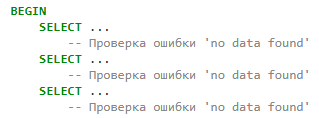
\includegraphics [scale=1] {my_folder/img/C1_code1.png}
	\caption{Пример кода с последовательной обработкой ошибок} 
	\label{fig:c1_code1}  
\end{figure}
\FloatBarrier

Если нам заранее известно, что имеется необходимость во всех данных из каждой команды SELECT, а при отсутствии хотя бы одних из них, мы должны выполнить какие-либо действия, то имеется возможность сильно упростить код, как показано на \firef{fig:c1_code2}.

\begin{figure}[ht!] 
	\center
	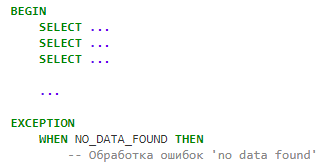
\includegraphics [scale=1] {my_folder/img/C1_code2.png}
	\caption{Пример обработки ошибок в отдельном блоке} 
	\label{fig:c1_code2}  
\end{figure}
\FloatBarrier

В таком случае обработка всех ошибок данного типа будет производиться в одном месте, отлаживать и дорабатывать такую программу будет гораздо проще, по сравнению с первым случаем. 
Также вынесение обработчика в отдельный блок, позволяет отделить логику работы основной программы, от раздела исключений, что позволяет уменьшить количество кода и повысить его читаемость.

В PL/SQL исключения бывают двух типов: системные и пользовательские. Системные исключения – это исключения, которые инициируются ядром PL/SQL в случае нарушением программы правил исполнения установленных Oracle. Пользовательские исключения, в свою очередь, определяются программистом и обычно связаны с конкретным приложением. 

Каждая ошибка имеет свой номер, но обрабатывать исключения можно только по их имени. В Oracle имеется несколько предопределенных ошибок, это часто возникающие ошибки, для которых заданно имя в пакете STANDARD. 

\begin{figure}[ht!] 
	\center
	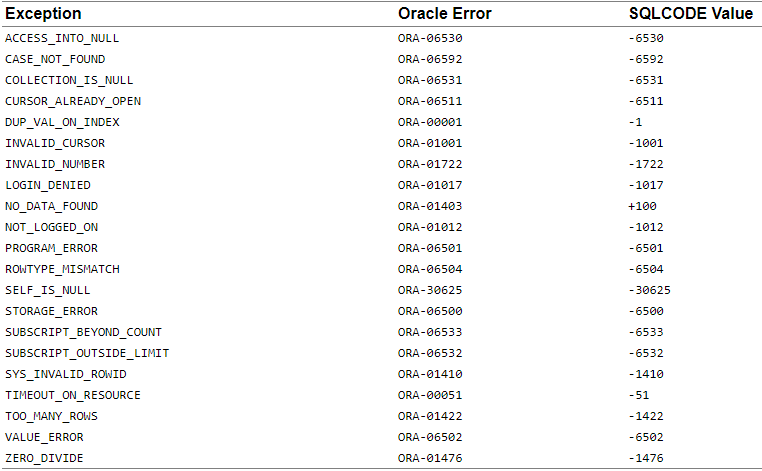
\includegraphics [scale=0.75] {my_folder/img/C1_tab1_predef_exceptions}
	\caption{Предопределенные ошибки из пакета STANDARD} 
	\label{fig:C1_tab1_predef}  
\end{figure}
\FloatBarrier

На \firef{fig:C1_tab1_predef}, приведены примеры предопределенных исключений. 

\section{Определение исключений} \label{ch1:sec2}
В подавляющем большинстве приложений определенных Oracle исключений недостаточно, поэтому необходимо уметь правильно определять и работать с пользовательскими ошибками, которые описывают исключительные ситуации для конкретного приложения.

\subsection{Объявление пользовательских исключений}

Пользовательские исключения позволяют программисту определить новые виды ошибок, для ситуаций, которые не покрываются системными исключениями. 

Очень важной особенностью пользовательских исключений является то, что взаимодейтсвие с ними не отличается от работы с системными ошибками. 

Определение именованных исключений похоже на объявление обычных переменных. Сначала указывается название ошибки, за которым следует ключевое слово EXCEPTION. 

\begin{figure}[ht!] 
	\center
	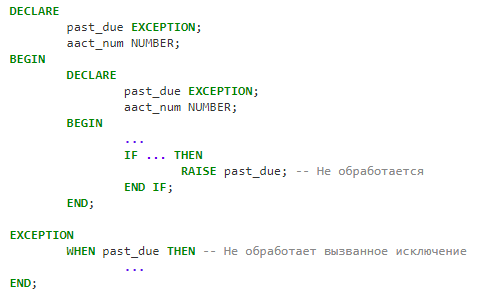
\includegraphics [scale=1] {my_folder/img/C1_exeception_declaration}
	\caption{Пример объявление именованного исключения} 
	\label{fig:C1_exeception_declaration}  
\end{figure}
\FloatBarrier

На \firef{fig:C1_exeception_declaration} показан пример объявления именованного исключения под названием past\_due. Во вложенном блоке объявляется еще одно исключение с таким же именем, так как вложенный блок не имеет обработчика, то его (локальное) исключение past\_due не будет обработано. Внешний блок ничего не знает об исключение past\_due из вложенного блока, поэтому его обработчик не сможет отловить и обработать данное исключение\cite{handling-errors}.

\subsection{Привязка исключений к кодам ошибок}

При помощи директив компилятора можно связать именованное исключение с кодом ошибки. Делается это при помощи команды EXCEPTION\_INIT, в которую передается имя исключения, объявленного ранее, и код ошибки. После такой привязки обращаться к ошибке в разделе WHEN можно по имени. 

Обычно данная директива используется в двух случаях: для задания имени системному исключению, для которого не предусмотренно предопределенного имени, и для работы со специфичными для приложения ошибками.

\begin{figure}[ht!] 
	\center
	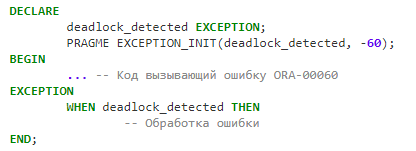
\includegraphics [scale=1] {my_folder/img/C1_exception_init}
	\caption{Пример использования директивы компилятора EXCEPTION\_INIT} 
	\label{fig:C1_exeception_init}  
\end{figure}
\FloatBarrier

В примере показанном на \firef{fig:C1_exeception_init} происходит привязка ошибки с номером -60 к именованному исключению deadlock\_detected.

Хорошим тоном считается вынесение часто используемых ошибок в один пакет и привязка их к номерам, как, например, это сделано в пакете STANDARD со стандартными исключениями. В таком случае, в остальном коде приложения, можно будет обращаться к ошибкам из данного пакета. Следуя такой практике можно повысить читаемость кода за счет стандартизации в определении ошибок.

\section{Инициирование исключительных ситуаций}\label{ch1:sec3}

Существует несколько способов инициировать исключение. В первую очередь, исключения инициируются Oracle в случае возникновения ошибки. Программист может сам инициировать исключения либо при помощи команды RAISE, либо используя процедуру RAISE\_APPLICATION\_ERROR. Рассмотрим последние два способа подробнее.
 
Команда RAISE останавливает нормальное выполнение программы PL/SQL и передает управление обработчику ошибок. Данная инструкция имеет следующий синтаксис.

\begin{figure}[ht!] 
	\center
	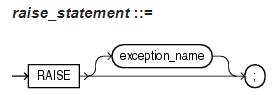
\includegraphics [scale=1] {my_folder/img/C1_raise_syntax}
	\caption{Синтаксис команды RAISE} 
	\label{fig:C1_raise_syntax}  
\end{figure}
\FloatBarrier

Как видно на \firef{fig:C1_raise_syntax} сначала указывается ключевое слово RAISE за которым следует необязательное имя исключения. 

Использование данной команды без указания имени исключения, можно только в разделе WHEN обработчика исключений. В таком случае обрабатываемое в данный момент исключение инициируется повторно, а процесс обработки исключения переходит в родительский блок. Это может быть полезно в случаях, когда нам нужно освободить какие-то ресурсы, либо сохранить какие-либо данные, но что делать с возникшей ошибкой в данный момент времени мы не знаем.

\begin{figure}[ht!] 
	\center
	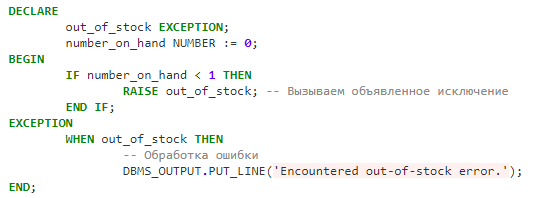
\includegraphics [scale=1] {my_folder/img/C1_raise_example}
	\caption{Пример использования команды RAISE} 
	\label{fig:C1_raise_example}  
\end{figure}
\FloatBarrier

На \firef{fig:C1_raise_example} представлен пример инициирования ошибки с использованием инструкции RAISE. В блоке происходит объявление исключения out\_of\_stock и переменной number\_of\_hand проинициализированной значением 0, после чего в условном блоке происходит проверка значения переменной, если оно меньше 1, то происходит инициирование объявленного ранее исключения, после чего исполнение передается блоку обработки ошибок. 

Другим способом инициировать программисту исключение является процедура RAISE\_APPLICATION\_ERROR из пакета DBMS\_STANDARD.

\begin{figure}[ht!] 
	\center
	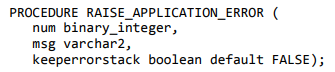
\includegraphics [scale=1] {my_folder/img/C1_raise_application_error_signature}
	\caption{Заголовок процедуры RAISE\_APPLICATION\_ERROR} 
	\label{fig:C1_raise_application_error_signature}  
\end{figure}
\FloatBarrier

Как видно на \firef{fig:C1_raise_application_error_signature} данная процедура может принимать три параметра, два обязательных и один необязательный. Первый параметр – это код ошибки, которую необходимо инициировать, в диапазоне от -20999 до -20000. Второй параметр – это сообщение длиной до 2048 байт, которое будет связано с ошибкой. Третий параметр keeperrorstack указывает, нужно ли добавить ошибку к уже имеющимся в стеке (данное поведение используется при указании значения TRUE), или необходим заменить существующую ошибку (значение FALSE, используемое по умолчанию).

\begin{figure}[ht!] 
	\center
	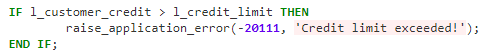
\includegraphics [scale=1] {my_folder/img/C1_raise_application_error_example}
	\caption{Пример использования процедуры RAISE\_APPLICATION\_ERROR} 
	\label{fig:C1_raise_application_error_example}  
\end{figure}
\FloatBarrier

Пример на \firef{fig:C1_raise_application_error_example} демонстрирует использование рассматриваемой процедуры. При нарушении бизнес-логики происходит инициирование ошибки с кодом -20111 с информацией об ошибке. 

\section{Обработка ошибок}\label{ch1:sec4}

При возникновении исключительной ситуации нормальное выполнение PL/SQL кода останавливается, а управление получает раздел обработки исключений, если обработчик данного блока не может справиться с такой ситуацией, то управление переходит в родительский блок. 

Синтаксис блока обработки исключений имеет следующий вид, показанный на рисунке \firef{fig:C1_exeception_handling_syntax}.

\begin{figure}[ht!] 
	\center
	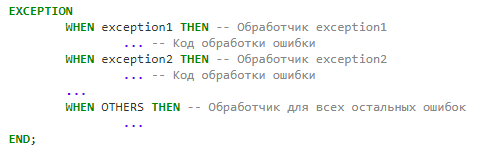
\includegraphics [scale=1] {my_folder/img/C1_exeception_handling_syntax}
	\caption{Синтаксис обработчика ошибок} 
	\label{fig:C1_exeception_handling_syntax}  
\end{figure}
\FloatBarrier

Он может находиться только в конце PL/SQL блока либо вовсе может отсутствовать. Если имя возникшего исключения совпадает с именем, указанным в разделе WHEN, то выполняются команды, находящиеся после ключевого слова THEN. В случае, когда ни один раздел с указанным именем не подходит управление переходит в раздел WHEN OTHERS, если он указан. 

Стоит отметить, что ошибка может быть обработана только одним из разделов. После выполнения команд управление передается в вызывающий блок. 


\section{Получение дополнительной информации об ошибке}\label{ch1:sec5}
Периодически, возникают ситуации, когда необходимо узнать дополнительную информацию об возникшей ошибке. В Oracle не существует возможности расширить объект EXCEPTION и записать туда свою информацию. В базе данных существует несколько функций, которые позволяют получить различную информацию из ошибки. К ним относятся: SQLCODE, SQLERRM, DBMS\_UNTILITY.FORMAT\_ERROR\_BACKTRACE и DBMS\_UNTILITY.FORMAT\_ERROR\_STACK. 
Рассмотрим каждую из них подробнее. 

Функция SQLCODE позволяет получить код возникшей ошибки, если вызвана в блоке обработки исключительных ситуаций, в том случае, если данная функция будет вызвана вне обработчика, то будет возвращено значение 0. Для ошибок, определенных пользователя, возвращается значение +1 или, если функции был присвоен код, при помощи директивы EXCRPTION\_INIT, то данный код и будет возвращен. 
При помощи данной функции можно обрабатывать исключения, которым не присвоены имена, по коду. Пример \firef{fig:C1_handling_by_sqlcode} показывает, как это можно сделать. 

\begin{figure}[ht!] 
	\center
	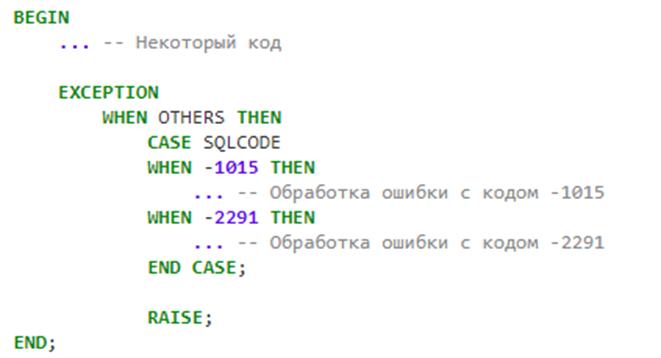
\includegraphics [scale=1] {my_folder/img/C1_handling_by_sqlcode}
	\caption{Обработка ошибок с использованием функции SQLCODE} 
	\label{fig:C1_handling_by_sqlcode}  
\end{figure}
\FloatBarrier

В данном примере, в обработчике ошибок происходит обработка всех ошибок. В случае заданных кодов выполняется особый код только для их обработки, после чего, при помощи команды RAISE снова возбуждается текущее исключение и передается в родительский код. 
Данную задачу можно было бы решить и другим способом, например, связать коды, для которых нужна особая обработка, с именами исключений, и указывать в конструкции WHEN их имена. Такой подход является более предпочтительным, но приведенный пример тоже имеет право на существование.

Функция SQLERRM возвращает сообщение ошибки, связанное с данным кодом. Может принимать в качестве параметра код ошибки. Если вызвана без параметров и в обработчике ошибок, то вернет ассоциированное с текущей ошибкой сообщение. 

Функция FORMAT\_ERROR\_STACK возвращает более подробную информацию об ошибке, в отличии от SQLERRM, помимо сообщения в вывод также включен текущий стектрейс ошибки. Стектрейс - последовательность вызовов и состояние окружения в некоторой точке программы. Преимуществом данной функции относительно SQLERRM является то, что SQLERRM строже ограничен в размерах сообщения. 

Функция FORMAT\_ERROR\_BACKTRACE позволяет получить стек вызова до точки, где была получена ошибка. Эта информация может потребоваться для нахождения причин ошибки. Например, после обработки ошибок, мы записываем в специальную таблицу полученный стек вызова. В дальнейшем, когда, нам будет необходимо исправить эту ошибку, мы можем обратиться к данной таблице и получить всю необходимую информацию о месте ее возникновения. 


\section{Логирование информации об ошибке}\label{ch1:sec6}
Большинство ошибок не может быть исправлено сразу, и не все ошибки требуют моментального исправления. Некоторые будут более приоритетными, некоторые менее, одни ошибки могут возникать очень часто, другие же встречаться крайне редко. Нужно правильно сохранять информацию об ошибках, когда придет время для ее исправления, мы должны иметь возможность получить максимум информации. Oracle предоставляет разработчикам пакет DBMS\_ERRLOG, в котором содержится одна процедура CREATE\_ERROR\_LOG. Данная процедура предназначена для логирования ошибок в DML операциях. 


\begin{figure}[ht!] 
	\center
	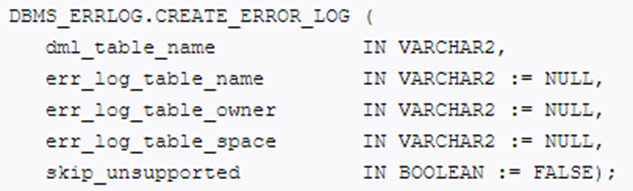
\includegraphics [scale=1] {my_folder/img/C1_create_error_log_syntax}
	\caption{Сигнатура процедуры DBMS\_ERRLOG.CREATE\_ERROR\_LOG} 
	\label{fig:C1_create_error_log_syntax}  
\end{figure}
\FloatBarrier

На рисунке \firef{fig:C1_create_error_log_syntax} представлена сигнатура данной процедуры. Процедура в качестве параметра принимает название таблицы, для которой производилась DML операция, информацию о таблице, в которую нужно занести информацию (таблица логирования) и флаг skip\_unsupported, который позволяет пропустить неподдерживаемые столбцы. К таким столбцам относятся колонки с типами данных LONG, CLOB, BLOB, BFILE и ADT. Если у флага указать значение FALSE, которое стоит по умолчанию, то в случае неподдерживаемого столбца, программа логгирования завершится. 

Данный пакет имеет ряд недостатков. Во-первых, он узконаправленный, сохранение информации об ошибках в не DML операциях, затруднено. Во-вторых, для логирования в нестандартную таблицу, потребуется каждый раз указывать много параметров. В-третьих, мы не можем контролировать информацию, которая будет заносится в таблицу. 

В связи с вышеперечисленным, разработчикам приходится разрабатывать собственный механизм для сохранения информации о возникающих ошибках, специализированный под нужды конкретного кода. 



\section{Выводы} \label{ch1:conclusion}
В ходе данной главы была рассмотрена основная информация об ошибках в PL/SQL. Были изучены инструменты для объявления пользовательских ошибок, для привязки исключительных ситуаций к кодам ошибок, были рассмотрены способы инициирования ошибок и их обработки.

При изучение существующих механизмов обработки ошибок в PL/SQL, были замечены некоторые недостатки и неудобства при работе с ними.  

%% Вспомогательные команды - Additional commands
%
\newpage % принудительное начало с новой страницы, использовать только в конце раздела
%\clearpage % осуществляется пакетом <<placeins>> в пределах секций
%\newpage\leavevmode\thispagestyle{empty}\newpage % 100 % начало новой страницы	         	 % Глава 1
\ContinueChapterBegin % размещать главы <<подряд>> 
\chapter{Обзор и анализ различных систем обработки исключительных ситуаций} \label{ch2}
	
% не рекомендуется использовать отдельную section <<введение>> после лета 2020 года
%\section{Введение} \label{ch2:intro}

Данная глава посвящена разбору существующих проблем в системе обработок ошибок, предлагаемой кампанией Oracle. 

В параграфе \ref{ch2:sec2} рассматриваются разработки разных авторов, нацеленные на решение схожих проблем. 

Про то, как происходит работа с исключительными ситуациями рассказывается в параграфе \ref{ch2:sec3}.
В параграфе \ref{ch2:sec4} приведен краткий обзор механизма взаимодействия с ошибками в объектно-ориентированных языках, на примере C\#.

Описание функциональных возможностей, которые необходимы в разрабатываемом пакете, перечисляются в параграфе \ref{ch2:sec5}.



\section{Существующие проблемы обработки ошибок}\label{ch2:sec1}
Несмотря на то, что существующая система имеет довольно много возможностей для разработчиков, она не лишена недостатков. Далее будут рассмотрены некоторые проблемы, с которыми сталкиваются программисты при разработке программного обеспечения для базы данных.

Дублирование кода. Довольно часто встречаются ситуации, в которых возможно возникновение одних и тех же ошибок, для обработки которой придется воспроизводить уже написанный код. Дублирование кода противоречит принципу разработки программного обеспечения DRY (Don’t repeat yourself, рус. не повторяйся), предложенного Энди Хайдом и Дэйвом Томасом в книге «Программист-прагматик»\cite{pragmatic}. Увеличение кодовой базы приводит к увеличению затрат ресурсов при отладке и корректировки приложения. Одним из способов решения данной проблемы является вынесение повторяющегося кода в отдельные процедуры или функции, и заменой повторяющегося кода на вызов необходимых подпрограмм. 

Очень явно данная проблема выражена при работе с пакетом UTL\_FILE, а конкретнее, с процедурой GET\_LINE. Данная процедура предназначена для извлечения строк из файлов, и в случае невозможности считать новую строку, будет выдано исключение NO\_DATA\_FOUND. Это приводит нас к тому, что каждый раз, когда нам необходимо считать данные из файла, мы должно написать код для обработки этой ошибки, который будет везде одинаковый. Данный код будет затруднять понимание основной логики, а допущенная ошибка при копировании кода, может привести к нежелательным последствиям\cite{utl-file}. 

\begin{figure}[ht!] 
	\center
	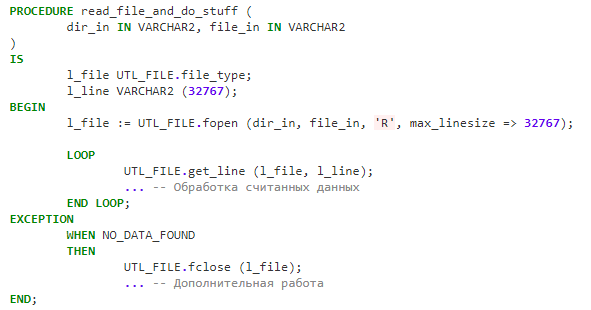
\includegraphics [scale=1] {my_folder/img/C1_utl_file_problem}
	\caption{Пример использования UTL\_FILE} 
	\label{fig:C1_utl_file_problem}  
\end{figure}
\FloatBarrier

На \firef{fig:C1_utl_file_problem} показан пример процедуры для чтения и обработки файла, с использованием пакета UTL\_FILE. Половину кода занимает обработчик ошибок, который должен присутствовать и обычно будет выполнять одну и ту же работу. Все это можно было бы сокрыть за одной функцией и работать с файлами при помощи вызова нужной подпрограммы, что займет всего одну строку кода, но позволит сократить количество ошибок и сэкономить время, затраченное на написание кода. В более сложных ситуациях, при которых использование процедуры такого вида невозможно по тем или иным причинам, все также можно будет воспользоваться пакетом UTL\_FILE.

Другой немаловажной проблемой при работе с ошибками является тот факт, что EXCEPTION в PL/SQL это особая разновидность структуры данных. Мы имеем достаточно небольшой набор возможностей для работы с ней, после объявления переменной данного типа, мы можем только инициировать или обрабатывать ее. Нету возможности для расширения функциональности данной структуры, мы не можем добавить дополнительные поля, мы не можем передавать исключения как параметр для процедуры или функции.

Также Oracle не дает возможностей для организации и классификации исключительных ситуаций, относящихся к конкретному приложению. В нашем распоряжении находиться 1000 кодов в диапазоне от -20999 до -20000. Разработчику необходимо следить чтобы коды использовались правильно, разные ошибки не должны связываться с одним и тем же кодом\cite{ferstein}. При боольшом количестве разработчиков это может быть затруднительно.

Для решения последних двух проблем можно реализовать альтернативную систему. Мы можем создать свои исключения и работать непосредственно с ними. Например, перечислить ошибки в отдельной таблице, тогда мы сможем передавать ошибки как параметры, дополнять всеми необходимыми для нас атрибутами, а необходимость контролировать это все перейдет от программиста к пакету, который будет этим заниматься. Под собственными ошибками будут скрыты исключения PL/SQL, в таком случае, мы, не потеряв преимуществ от работы со стандартных исключениями, будем иметь возможность при необходимости расширить их функциональность\cite{kite}. 

Дополнить такой пакет можно множеством различных способов, мы имеем полный контроль над аудитом ошибок, и можем его корректировать под свои нужды, в зависимости от приложения, можно собирать необходимый контекст возникновения ошибки и дополнять его при необходимости. Расширение пакета подпрограммами для обработки часто возникающих исключительных ситуаций позволит избежать проблемы дублирования кода. 


\section{Альтернативные возможности для обработки исключительных ситуаций}\label{ch2:sec2}

С обозначенными проблемами сталкивались и другие разработчики. Рассмотрим какие существуют способы улучшения процесса обработки ошибок. 

Стивен Ферштейн в своем докладе \cite{BestPracticePLSQL} про хорошие практики программирования на PL/SQL упоминает про Quest Error Manager (QEM). Получить много информации о нем не удалось, так как его перестали обновлять еще в 2010 году. Удалось выяснить, что этот довольно старый пакет, разработанный кампанией Quest, предназначался для решения схожих проблем. Установлено, что целью данного пакета было упрощение логирования информации об ошибках. 

В книге \cite{ferstein} Ферштейн и Прибыл выделяют похожие трудности при работе с исключительными ситуациями, и для изучения предоставляют пакет для обработки ошибок. Они говорят о том, что пакет не дописан и требует улучшений со стороны читателей, и предлагают выполнить это в качестве упражнения. Это небольшой пакет, состоящий всего из трех функций, предназначенный для демонстрации того, каким образом можно обрабатывать исключительные ситуации, альтернативным от стандартного способом. 

В ходе поиска существующих решений, было замечено, что во многих компаниях разрабатываются собственные пакеты для упрощения работы с обработчиками ошибок, но так как эти разработки являются собственностью кампаний, в открытом доступе их нет. 


\section{Механизмы обработки ошибок в других базах данных}\label{ch2:sec3}

Рассмотрим, как исключительные ситуации обрабатываются в других базах данных. 

В базе данных MySQL схема обработки ошибок довольно сильно схожа с той, которая применяется в Oracle Database. Здесь используются обработчики, которые, по своей сути, не отличаются от блока обработки ошибок в PL/SQL. Используется сигнальная схема, исключения именуются сигналами, тоже привязываются к кодам ошибок. Сигналы могут содержать дополнительную информацию об возникшей проблеме, которую можно указать при вызове сигнала, таковой информацией является: каталог, схема и имя ограничения, каталог, схема, колонка и название таблицы, имя курсора. 

Обработчики бывают разных типов, например, continue и exit. Они отличаются тем, что будет происходить, после того как сигнал обработается. 

В целом, такая система мало отличается от системы принятой в Oracle Database, и подвержена тем же проблемам, но имеет ряд возможностей упрощающих работу с ошибками и ускоряющих процесс написания кода\cite{MySqlDocumentation}.

Процедурный язык Transact-SQL, являющийся расширением языка SQL, разрабатывается кампанией Microsoft. Данный язык используется в базах данных SQL Server и Sybase.
В Transact-SQL исключительные ситуации обрабатываются посредством блока TRY…CATCH. Вызов ошибок происходит посредством команды RAISERROR, в которую передаются системные параметры ошибки, такие как код, сообщение, важность и положение.  Последний параметр позволяет конкретизировать место возникновение ошибки, если возникло несколько одинаковых ошибок в разных местах\cite{TSQLDocumentation}.

В базе данных PostgreSQL то, как вы будете обрабатывать ошибки, зависит от используемого языка процедурного расширения. Согласно документации, PL/pgSQL очень схож с процедурным языком Oracle PLSQl\cite{PostgreSqlDocumentation}.

Действительно, синтаксис работы с ошибками, мало отличается. Используются такие же конструкции для блока обработки, обращаться к ошибкам можно по имени или коду. Можно получать расширенную информацию об ошибке, схожую с информацией, передаваемой с событиями в MySQL. 

В общем, обработка исключений работает схоже в разных базах данных. Везде имеется завязка на коды ошибок, корректную работу с которыми должен контролировать программист. Расширение объектов типа EXCEPTION ограничено или вовсе отсутствует. 

\section{Примеры обработки ошибок в объектно-ориентированных языках}\label{ch2:sec4}

Рассмотрим, как происходит работа с исключительными ситуациями в других языках программирования. Рассматривать будем язык C\#. Изучим пример, приведенный на рисунке \ref{fig:C2_c_sharp_user_defined_exceptions}. 

\begin{figure}[ht!] 
	\center
	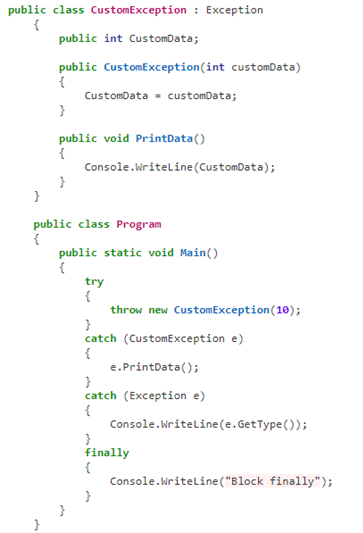
\includegraphics [scale=1] {my_folder/img/C2_c_sharp_user_defined_exceptions}
	\caption{Пример обработки ошибок в C\#} 
	\label{fig:C2_c_sharp_user_defined_exceptions}  
\end{figure}
\FloatBarrier

В данном коде объявляется пользовательская исключительная ситуация CustomException, она наследуется от базового класса Exception. В данном объекте мы объявляем переменную CustomData для хранения необходимой информации, а также метод PrintData, для вывода данной информации в консоль. 

Далее, в классе Program, в методе Main, происходит основная работа программы. Блок try/catch позволяет выполнить код, и в случае возникновения ошибки обработать ее. Мы имеем возможность выполнить различный код, в зависимости от ошибки, указывая несколько блоков catch (схожим образом мы разделяем обработку разных ошибок в PL/SQL). Аналогом блока try/catch в PL/SQL будет являться объявление вложенного блока begin/end с указанием ключевого слова exception. 

В коде, расположенном в блоке try создается экземпляр класса пользовательской ошибки, с указанием конкретных данных, в данном случае числа 10, и происходит вызов данного исключения, при помощи ключевого слова throw. В операторе catch выполняется обработка данной ошибки, вызывается созданный нами метод, который выведет информацию на консоль. 

Также, в данном примере, используется ключевое слово finally. Код, расположенный в данном блоке, выполнится независимо от того возникло какое-либо исключение или нет. Данная функциональность обычно используется для корректного завершения работы кода из блока try, например, для закрытия файлов, которые были ранее открыты.

В результате выполнения данного примера, на консоль будет выведенно две строки, первая, с числом 10, и вторая со строкой "Block finally".

Данный подход к работе с исключительными ситуациями не накладывает на нас ограничений, которые существуют в PL/SQL. Программисту не нужно следить за кодами ошибок, имеется достаточное количество предопределенных классов, с различными ошибками, мы можем спокойно передавать любое количество данных. Современные IDE подскажут разработчику какие исключения созданы, и уже из представленного списка, можно будет выбрать подходящее.

В других объектно-ориентированных языках взаимодействие с исключительными ситуациями происходит схожим образом. 


\section{Требования к разрабатываемому пакету}\label{ch2:sec5}

Среди выдвинутых проблем при обработке ошибок, особенно выделяется неудобство взаимодействия с кодами ошибок. Разработчики продукта обязаны самостоятельно контролировать и следить за тем, какие коды использованы, какие свободны, какой номер ошибки нужно применить в той или иной ситуации. Не редко для этих целей используется документ, в котором программисты составляют перечень номеров, которые уже используются. 
Для решения этой проблемы в пакете будет присутствовать таблица, содержащая подробную информацию об каждой ошибке. В которую входит: код ошибки, тип ошибки, имя для исключения, подробное описание исключительной ситуации, информация об области применения, дополнительная информация, специфичная для пользователей пакета. 

Особенно важной функциональностью для такого пакета является функциональность сохранения информации об возникающих ошибках. А также различные представления, предоставляющие удобный способ для анализа ошибок. Должна быть собрана информация об частотности возникновения ошибок, местах их появления, данных, которые привели к возникновению ошибке такого рода. 

Для избавления проблем с дублированием кода, будут предусмотрены несколько стандартных методов-обработчиков ошибок, с возможностью расширить тот список пользовательскими обработчиками. Среди стандартных обработчиков должны присутствовать:

\begin{enumerate}
\item Обработчик с логированием и повторным возбуждением исключения, заносящий информацию в специальное место, и передающий ошибку в вызывающий блок. 
\item Обработчик с логированием и сокрытием ошибки, данный метод будет сохранять информацию и завершать выполнение блока, в котором возникло исключение, без передачи ошибки дальше. 
\item «Тихие» обработчики, данные обработчики схожи по функционалу с предыдущими, но не производят логирования об возникшей ошибке. 
\item Обработчик критических ошибок, такой метод предназначен для работы с особо важными ошибками, затрагивающими основную логику приложения. Помимо занесения информации в стандартные места, данная процедура позволит сообщить администратору об возникновении критической ситуации, через другие каналы связи, например по почте. Функционал для настройки оповещения будет предусмотрен в разрабатываемом пакете. 
\end{enumerate} 


Необходима возможность для настройки параметров пакета, так называемые feature flag. Это поля (обычно содержащие бинарное значение), позволяющие включить или отключить, ту или иную функциональность. 

Данный список требований будет пополнен функциональными возможностями, необходимость в которых возникнет в ходе разработки.

\section{Выводы} \label{ch2:conclusion}
В ходе данной главы были рассмотрены проблемы, которые затрудняют разработку продуктов на языке Oracle PL/SQL. Были предложены различные способы для их устранения.
Был проведен разбор пакетов, упрощающих работу с исключительными ситуациями. Также было рассмотрено как обработка ошибок реализована в других СУБД. 
После этого были выдвинуты требования к реализуемому пакету, с описанием того, как та или иная функциональность способствует решению обозначенных проблем. 




%% Вспомогательные команды - Additional commands
%
\newpage % принудительное начало с новой страницы, использовать только в конце раздела
%\clearpage % осуществляется пакетом <<placeins>> в пределах секций
%\newpage\leavevmode\thispagestyle{empty}\newpage % 100 % начало новой страницы	         	 % Глава 2
\chapter{Разработка пакета} \label{ch3}

В данной главе рассматривается различные этапы создания пакета. Начиная с разработки и выбора алгоритма работы с ошибками, заканчивая созданием скриптов для создания и удаления пакета.

 
\section{Настройка среды} \label{ch3:sec1}

Для разработки будет использоваться база данных Oracle версии 11g Release 2. Установленная в виртуальную машину Oracle VirtualBox, под управлением ОС Windows Server 2008. Дополнительно нужно установить схемы примеров, предоставляемые Oracle (в дальнейшем потребуется для тестирования), а также пакет UTL\_MAIL для отправки Email сообщений, который поставляется с базой, но не установлен по умолчанию. В качестве среды разработки будем использовать Oracle SqlDeveloper и JetBrains DataGrip. Создадим пользователя, от лица которого будем разрабатывать пакет. 

\begin{figure}[ht!] 
	\center
	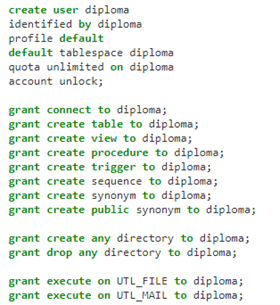
\includegraphics [scale=1] {my_folder/img/C3_create_user.png}
	\caption{Код создания пользователя и выдачи привилегий} 
	\label{fig:C3_create_user}  
\end{figure}
\FloatBarrier

На \firef{fig:C3_create_user} представлен скрипт создания пользователя и выдачи привилегий. Пользователю потребуются: привилегия на создание подключения, создание таблиц, представлений, синонимов и публичных синонимов, последовательностей, процедур и триггеров, привилегии для создания и удаления директорий, а также привилегии на работу с пакетами UTL\_FILE и UTL\_MAIL. 

Данный пользователь предназначен только для разработки, пользователям пакета не нужно будет создавать такого пользователя, поэтому использование некоторых потенциально опасных привилегий (например, drop any directory) является допустимым. Если в ходе разработки потребуются дополнительные разрешения, об этом будет специально указано.


\section{Структура распространяемого пакета} \label{ch3:sec2}

Пакет будет распространяться как SQL скрипт, который состоит из установщика и скриптов самого пакета. Инсталлер выполняет работу по созданию основных объектов, таблиц, триггеров, последовательностей, представлений. После чего производится вставка данных, в основные таблицы, сюда входит информация о базовых ошибках, описание их типов, создание параметров и выставление их в значения по умолчанию. Так же установочный скрипт занимается созданием директории для логирования файлов.


\section{Схема хранения информации} \label{ch3:sec3}

Первоначально, для решения проблемы работы с кодами ошибок, необходимо сокрыть их использование за процедурами пакета. Опишем сущность исключительной ситуации, с которой будем работать в дальнейшем. 

Для ошибки нам необходимо хранить следующую информацию: код ошибки, наименование ошибки, тип ошибки и информацию о ней, а также дополнительную мета информацию, в которую будет входить, временная метка создания записи об ошибки, и имя пользователя, который создал данную ошибку. Номер ошибки (код) будет использоваться в ходе работы пакета, для упрощения идентификации, пользователи же будут использовать наименования ошибки, так как правильно выбранное имя, более подробно описывает суть ошибки и проще для запоминания человеком, но, в случае необходимости, пользователи все также могут обращаться к ошибкам по кодам. Это позволит сделать разрабатываемый пакет расширяемым, не скрывая от пользователей всех возможностей. 

Данная информация будет храниться в таблице ERRM\$ERRORS, которая будет связана с таблицей ERRM\$ERROR\_TYPES. Таблица ERRM\$ERROR\_TYPES будет содержать описание типов исключительных ситуаций. Типы позволят разделить ошибки на группы, и обрабатывать ошибки по-разному в зависимости от их важности. Информация, хранящаяся о категориях, подобна той информации, которую мы храним об ошибках, здесь содержится ID типа, наименование типа и информация о нем. 

Модель хранения данных, используемая в пакете, представлена на \firef{fig:C3_er_model}.

\begin{figure}[ht!] 
	\center
	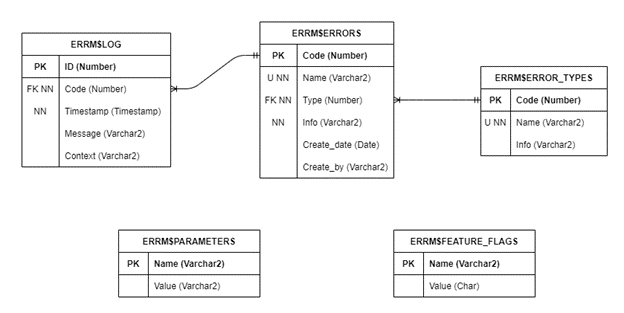
\includegraphics [scale=1] {my_folder/img/C3_er_model.png}
	\caption{ER модель хранения информации пакета} 
	\label{fig:C3_er_model}  
\end{figure}
\FloatBarrier

Здесь и далее, для Entity-relationship моделей используются следующие обозначения: PK – первичный ключ (Primary Key), FK – внешний ключ (Foreign Key), U – уникальное поле (Unique), NN – обязательное поле (Not null). 

Таблица ERRM\$ERRORS имеет ссылочное ограничение на первичный ключ таблицы ERRM\$ERROR\_TYPES. 
Возникающие в ходе работы приложения, ошибки необходимо хранить для дальнейшего анализа, для данных целей присутствует таблица ERRM\$LOG, в которую заносится номер записи, код ошибки (имеется связь с таблицей ERRM\$ERRORS), временная метка возникновения ошибки, сообщение, а также контекст данной ситуации. 

Здесь, и в дальнейшем, под контекстом ошибки понимается набор именованный набор данных, если не сказано иного.  

Дополнительно, присутствуют две таблицы для задания параметров пакета, это ERRM\$PARAMETERS и ERRM\$FEATURE\_FLAGS. Вторая таблица хранит установленные значения опций, то есть тех настроек, которые имеют бинарное значение (включена/выключена), например возможность логирования информации в файл. А первая отвечает за настройку не бинарных параметров, например, название файла для записи информации об ошибках, почта администратора. 


\section{Дополнительные объекты для обработки информации} \label{ch3:sec4}
 
Помимо перечисленных в параграфе \ref{ch3:sec3} таблиц, нам необходимы дополнительные объекты базы данных, которые будут обеспечивать целостность и корректность хранимой информации.

Первая категория - это последовательности. Последовательность – это объект базы данных, предоставляющий пользователю последовательность чисел по указанным правилам. Нами будет использоваться три последовательности. Первая – для кода ошибок, вторая – для номера типов ошибок, и третья – для последовательного номера записи в таблице логирования.  

Во вторую категорию попадают триггеры на таблицы. Для таблиц ERRM\$PARAMETERS и ERRM\$FEATURE\_FLAGS за счет триггеров будет контролироваться вид хранимой информации, все имена параметров должны храниться в верхнем регистре, а значения параметров - в нижнем, значения для feature flag должны быть либо символом 0, либо символом 1. В случае, если пользователи будут добавлять некорректные данные, триггер не позволит вставить такую информацию, обновление информации будет отклонено, возникнет исключение с сообщением. 


\section{Определение спецификации пакета} \label{ch3:sec5}
 
Весь пакет (спецификация и тело) будет образно разделен на подкатегории, таким образом пользователям будет проще ориентироваться в пакете, читаемость кода такого пакета будет выше. Были выделены следующие категории структуры пакета: 

\begin{enumerate} 
\item CONSTANTS – в данном блоке будут объявляться константные значения пакета
\item TYPES – объявление используемых типов данных
\item PARAMETERS WORK – процедуры и функции для настройки параметров пакета
\item HELPERS – дополнительные действия 
\item PROCEDURE AND FUNCTIONS – методы для основной работы с пакетом
\item SILENT RAISES – методы для вызова исключений без логирования
\item LOG WORK – процедуры работы с местами хранения логов
\item SIMPLE ERROR RAISE – процедуры для упрощения вызова часто используемых ошибок
\item LOG – блок для вывода информации на экран, упрощение работы с пакетом DBMS\_OUTPUT
\end{enumerate} 

В коде пакета данные категории будут помечены комментариями и разделяться пустыми строками. Данное разделение является условным и на работу программы не влияет. 

Выделим типы, с которыми будем работать. Объявив типы (или подтипы, как в нашем случае) мы сможем отвязаться от конкретного способа хранения данных, и, в случае, когда тип нужно будет изменить, например если код ошибки потребуется хранить не числом, а строкой, это сделать будет очень просто, поменяв объявление типа в спецификации пакета. Мною были объявлены следующие типы данных:

\begin{enumerate} 
\item t\_err\_code – тип для идентификации ошибки, является подтипом типа pls\_integer 
\item t\_err\_name – тип для работы с именем ошибки, подтип varchar2 размером в 100 символов.
\item t\_err\_type – тип для хранения категории ошибки, наследуется от типа pls\_integer
\end{enumerate} 

Для возможности настройки параметров пакета нам потребуется, как минимум, 4 метода. Получение и задания значений параметров, а также получений и задание флагов возможностей. Оба метода на получение установленного значения будут принимать один входной параметр – имя настройки, а возвращать сохраненное в таблице значение, отличие будет в возвращаемом типе данных, для параметров это будет строка (varchar2), для опций это Boolean. 

Так же для работы с опциями и параметрами объявим несколько строковых констант, в которых будут сохранены имена для параметров. Это позволит пользователям не заботиться о правильности написания названия того или иного параметра, а просто обратиться к константе. 

Для констант будут использоваться следующие префиксы: FEATURE\_ для бинарных опция (которые хранятся в таблице ERRM\$FEATURE\_FLAGS, подробнее смотри в параграфе \ref{ch3:sec3}) и PARAMETER\_, собственно, для параметров (хранятся в таблице ERRM\$PARAMETERS). При помощи этих префиксов будет понятно, какие методы нужно использовать, и какое значение мы ожидаем в результате работы функции. 

\begin{figure}[ht!] 
	\center
	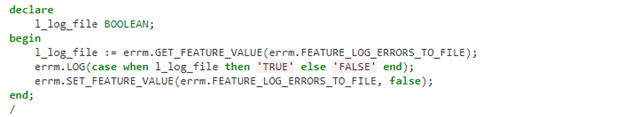
\includegraphics [scale=1] {my_folder/img/C3_get_feature.png}
	\caption{Пример получения и установки значения опции} 
	\label{fig:C3_get_feature}  
\end{figure}
\FloatBarrier

На \firef{fig:C3_get_feature} показан пример использования описанных ранее процедуры и функции для работы с опциями. В данном анонимном блоке объявляется бинарная переменная, в которую заносится значение опции FEATURE\_LOG\_ERRORS\_TO\_FILE, которая отвечает за логирование в файл. После чего происходит вывод информации на экран, при помощи метода LOG (о нем будет сказано далее), затем происходит отключение возможности логирования в файл.

Использование констант также защищает пользователей от дополнительных ошибок, если бы пользователю пришлось задавать название параметра вручную, велика вероятность опечатки, и в результате мы получим ошибку на этапе исполнения, когда программа сделает запрос к таблице и не найдет параметра с таким значением. В случае же использования констант среда разработки подскажет, какие константы мы можем использовать, но даже в случае опечатки, ошибка возникнет еще на этапе компиляции, что позволит заметить ее гораздо раньше, и исправить. При этом функции GET\_FEATURE\_VALUE и GET\_PARAMETER\_VALUE принимают строки, что дает возможность пользователям, в случае необходимости, обратиться к значениям настроек на прямую, без использования констант. 

Методы для вывода информации из категории LOG, сюда входит две процедуры LOG (которая уже использовалась ранее) и NL. Данные методы являются обертками для вызовов стандартных методов из пакета DBMS\_OUTPUT. Процедура LOG работает аналогично, процедуре PUT\_LINE, а процедура NL скрывает за собой процедуру NEW\_LINE. Это упрощает написание кода для отладки, и позволяет с легкостью заменить вывод отладки, например, на вывод в файл, достаточно будет поправить только один метод. Нет нужды заставлять пользователей использовать данные методы, так как не известно как конкретно работает логирование в пользовательском приложении, довольно вероятна ситуация, когда используется другой пакет, например, log4plsql (популярный фреймворк для логирования информации, предоставляет множество различных мест логирования, поддерживает Oracle Forms, Oracle Report\cite{log4plsql}), но для удобства они были вынесены в спецификацию.

В категорию HELPERS входит единственный метод GET\_ERROR\_CODE, который позволяет по имени ошибки получить ее код. Методы для пользователей имеют определения как для работы с кодами ошибок, так и для работы с именами ошибок (что является более предпочтительным), но данная функциональность может потребоваться пользователям пакета. Допустим, что имеется необходимость не вызывать ошибку прямо сейчас, а требуется записать ошибку, либо передать ее куда-то, выполнить дополнительную работу (собрать расширенный контекст ошибки), и только потом вызвать исключение, в таком случае можно сохранить (или передать в другой метод) имя ошибки, в котором произойдет необходимая работа, после чего, при помощи данного метода происходит получение кода ошибки, проводятся дополнительные операции с ошибкой, и в итоге происходит вызов ошибки. Суммируя, данная функциональность расширяет перечень возможностей пакета. 

Рассмотрим процедуры для работы с местами логирования информации (категория LOG WORK). Сюда включены две процедуры CLEAR\_LOG\_TABLE и CLEAR\_LOG\_FILE. Как понятно из их названия, они предназначены для очистки хранилища ошибок, таблицы или файла, соответственно. 

Далее будут рассмотрены методы для основной работы с пакетом. 

Процедура REGISTER\_ERROR предназначена для создания ошибки, за ней будет скрываться вставка данных в таблицу ERRM\$ERRORS, предваренная дополнительными действиями, генерация кода ошибки, если он не указан, приведение имени ошибки к стандартному имени и так далее. На вход процедура принимает: код ошибки, не обязательный параметр, наименование ошибки (обязательно), тип ошибки (не обязательно, по умолчанию устанавливается обычная ошибка), информация об ошибке (обязательно), комментарий про использование данного вида ошибки. Информация об ошибке фактически не является обязательным параметром, но будем обязывать пользователей ее указывать, чтобы при возникновении ошибки была максимально понятна ее суть. Поля с датой создания и именем пользователя-создателем, будут обновляться при помощи триггера. 
Для вызова ошибки будут использоваться методы RAISE, всего таких методов будет 4. Первый (самый предпочтительный вариант) принимает в параметрах имя вызываемой ошибки, и не обязательный флаг p\_log\_enabled, который отвечает за необходимость логирования информации об ошибке. Второй метод, принимает вместо имени код ошибки, имеет аналогичный второй параметр. В обоих этих методах параметр p\_log\_enabled не является обязательным и по умолчанию имеет значение true, что означает, что логирование будет производиться. 

Остальные два метода имеют префикс s (сокращение от слова silent(англ.) – тихий), итоговое название SRAISE, они вызывают обычный метод raise, с установкой второго параметра в значение false. Что означает, что логирование производиться не будет. Данный обработчик используется в тех случаях, когда нужно прервать выполнение программы, но не требуется заносить информацию об этом. Данные методы, по умолчанию, принимают имя ошибки в качестве параметра, но имеет перегрузку процедуры, в которой задается номер ошибки, вместо имени. 

В категорию SIMPLE ERROR RAISE попадают процедуры, которые позволят вызвать исключение одной строчкой, не нужно знать даже наименование ошибки, что очень удобно для часто используемых исключительных ситуаций. В данный момент, сюда включено 4 метода, для заранее предопределенных ошибок: DEFAULT\_ERROR, DEFAULT\_LOG, DEFAULT\_WARNING и NOT\_IMPLEMENTED\_EXCEPTION. Первые три представляют собой вызов стандартных (для данного пакета) исключительных ситуаций с разными типами (подробнее смотри в параграфе \ref{ch3:sec3}), последний является вызовом ошибки, которая гласит, что код еще не реализован. 

Рассмотрим пример, пользователь разрабатывает пакет, определил спецификацию и реализовал в теле не все методы, но имеется желание уже протестировать работу данных процедур и/или функций. Для нереализованных методов можно создать простую реализацию с заглушкой состоящей из одной команды null, которая не выполняет никаких действий, но такая ситуация является опасной, если метод так и не будет реализован, то при вызове этих методов ничего не произойдет, проблема заключается в том, что об этом никто не узнает, пользователь, вызывая код на исполнение, ожидает, что метод выполнит свою работу, но этого не происходит. Если же использовать исключение, то при вызове данного метода, сразу станет понятно, что метод еще не готов, и использовать его еще рано. Так же это упростит процедуру автоматического тестирования, так как нам будет сразу известно, что метод не выполнил работу, и нам нет нужды производить более сложную проверку. 

Рассмотрим, как будет проходить взаимодействие пользователей с контекстом ошибок. Для этого в пакете предусмотрены две процедуры ADD\_CONTEXT и CLEAR\_CONTEXT. Первая добавит к контексту дополнительную информацию, принимает два строковых параметра: название и значение. Вторая очищает значения в сохраненном контексте. Контекст автоматически очистится после вызова ошибки.

\begin{figure}[ht!] 
	\center
	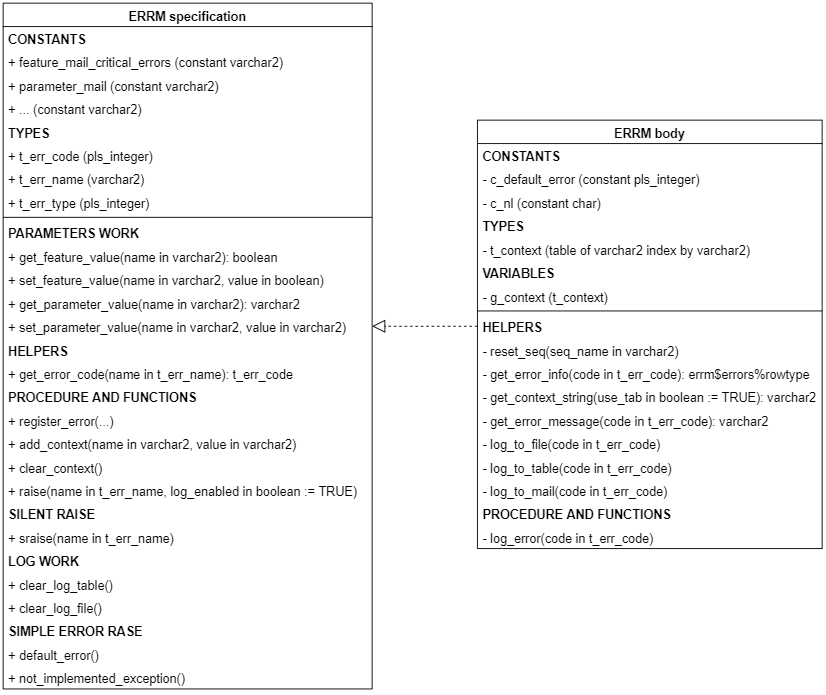
\includegraphics [scale=0.6] {my_folder/img/C3_UML_diagram.png}
	\caption{UML диаграмма пакета} 
	\label{fig:C3_UML_diagram}  
\end{figure}
\FloatBarrier

На \firef{fig:C3_UML_diagram} представлена схематичная UML диаграмма пакета, на ней показаны не все, а только основные процедуры и функции. В теле пакета указаны только методы, отличные от спецификации пакета, остальные методы, тоже будут реализованы. Категории блоков пакета выделены жирным. 


\section{Создание установщика} \label{ch3:sec6}

Весь пакет состоит из четырех файлов: установщик, определение спецификации пакета, определение тела пакета, деинсталлер. Установщик занимается созданием и настройкой необходимых объектов, после чего запускает скрипты для создания пакета. В итоге три первых скрипта могут быть объединены в один, для исключения лишних ошибок. 

Рассмотрим принципиально важные моменты создания установщика. Все начинается с создания таблицы типов ошибок ERRM\$ERROR\_TYPES. Код этой части инсталлера представлен на  \firef{fig:C3_create_error_types_table}.

\begin{figure}[ht!] 
	\center
	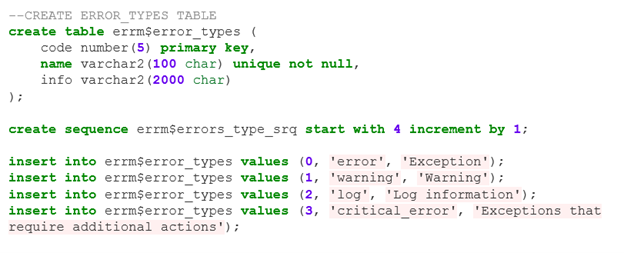
\includegraphics [scale=1] {my_folder/img/C3_create_error_types_table.png}
	\caption{Код создания таблицы типов} 
	\label{fig:C3_create_error_types_table}  
\end{figure}
\FloatBarrier

Первоначально создается таблица для хранения типа ошибок, затем создается последовательность для хранения кодов типов, после чего производится вставка нескольких базовых типов. 

\begin{figure}[ht!] 
	\center
	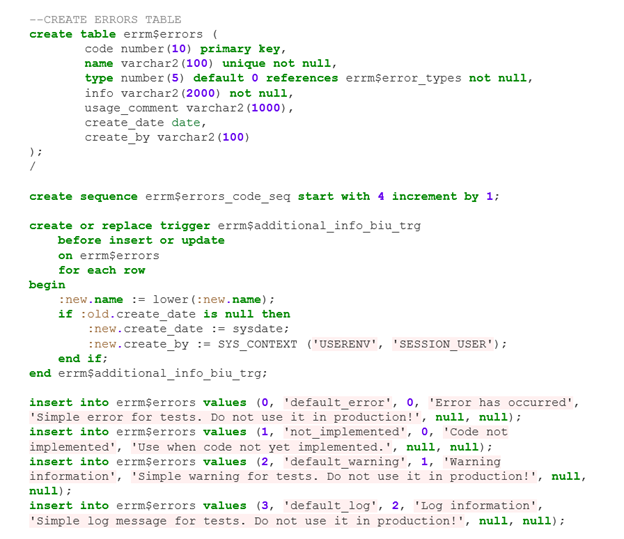
\includegraphics [scale=1] {my_folder/img/c3_create_errrors_table.png}
	\caption{Код создания таблицы ошибок} 
	\label{fig:c3_create_errrors_table}  
\end{figure}
\FloatBarrier

На \firef{fig:c3_create_errrors_table} представлен код создания таблицы ошибок, создания последовательности. 

Создается триггер, который приводит имя ошибки к стандартному виду и добавляет мета информацию при создании новой записи. Для этого используется стандартная процедура SYS\_CONTEXT, которая позволяет получить имя пользователя. 

\begin{figure}[ht!] 
	\center
	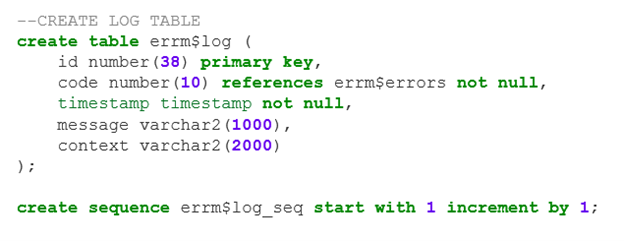
\includegraphics [scale=1] {my_folder/img/C3_create_log_table.png}
	\caption{Код создания таблицы для логирования} 
	\label{fig:C3_create_log_table}  
\end{figure}
\FloatBarrier

На \firef{fig:C3_create_log_table} показан код создания таблицы для хранения логов ошибки, и последовательности, для нумерации логов.

Код для создания остальных таблиц ERRM\$PREFERENCES и ERRM\$FEATURE\_FLAGS, а также триггеров и данных, можно посмотреть в приложении \ref{appendix-1}. 


\section{Разработка тела пакета} \label{ch3:sec7}

Далее будут подробно описаны принципиально важные участки пакета, менее важные моменты рассмотрены не будут, полный код пакета содержится в приложении \ref{appendix-1}.

Схематичный алгоритм вызова исключения представлен на \firef{fig:c3_block_diagram}. 

\begin{figure}[ht!] 
	\center
	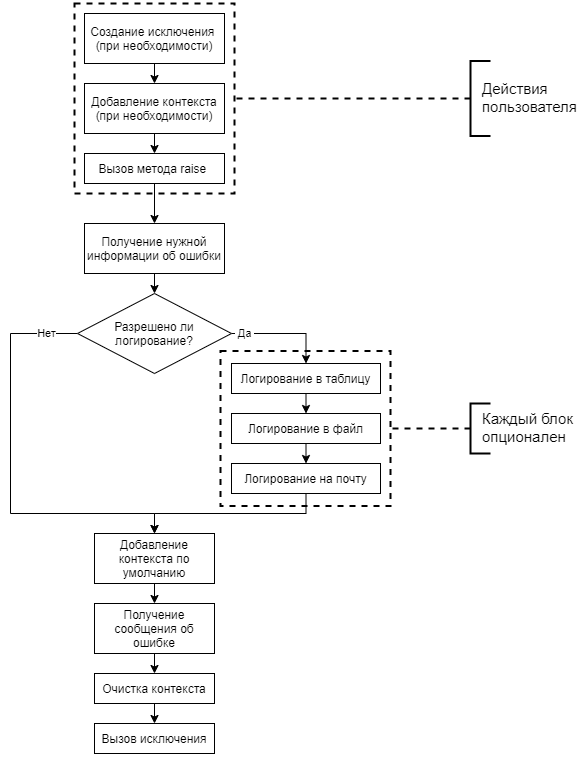
\includegraphics [scale=1] {my_folder/img/c3_block_schema.png}
	\caption{Блок схема вызова исключения} 
	\label{fig:c3_block_diagram}  
\end{figure}
\FloatBarrier

Первые операции (выделенные в блок) выполняет пользователь, остальное скрыто за реализацией пакета. В случае логирования информации об ошибке, каждая процедура для логирования информации в определенное место (например, на почту), проверяет доступность этого метода согласно установленным значениям опций пакета. 

Вызов исключения всегда происходит с определенным кодом, который задается при создании тела пакета, используется значение -20000, зарезервированное Oracle для пользовательских приложений. Данное значение вынесено в константу, при необходимости использовать другой код, пользователи могут заменить номер в теле пакета. Вызов исключения происходит при помощи стандартной процедуры RAISE\_APPLICATION\_ERROR, в которую передается указанный код, а также отформатированное сообщение об ошибке, в нем указывается название и код исключительной ситуации из пакета, краткое описание ошибки, тип ошибки и контекст. В случае, если включено все логирование эта же информация заносится в таблицу ERRM\$LOG, и в файл логирования. Если возникшая ошибка является критической, происходит отправка письма администратору, почта которого задается в параметрах пакета. 

Данное описание справедливо для процедуры RAISE принимающей код ошибки. 

Все остальные методы для возбуждения исключения (RAISE с именем ошибки, два вида SRAISE, упрощенные методы для вызовы часто используемых ошибок) сводятся к вызову основного метода RAISE.

\begin{figure}[ht!] 
	\center
	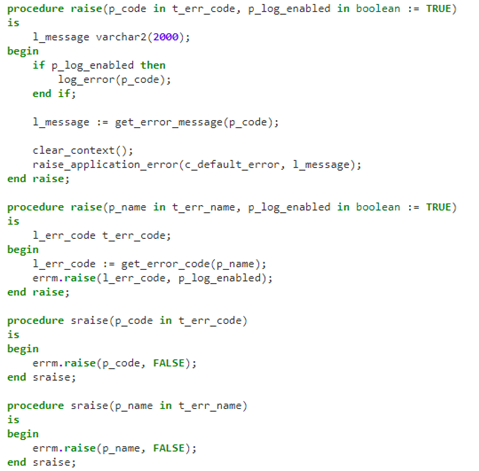
\includegraphics [scale=1] {my_folder/img/c3_raise_code.png}
	\caption{Код метода Raise} 
	\label{fig:c3_raise_code}  
\end{figure}
\FloatBarrier

Код процедуры RAISE и того, как остальные процедуры завязаны на основной метод представлен на \firef{fig:c3_raise_code}. 

Методы для упрощенного вызова ошибок работают следующим образом: вызывается метод RAISE c указанным в методе кодом ошибки. Для расширения перечня таких методов пользователи могут добавить аналогичные методы, либо в данный пакет и перекомпилировать его, либо в какое-либо свое пространство. Данное действие рекомендуется провести для всех часто используемых ошибок. 

Для логирования информации об ошибке основной метод RAISE вызывает процедуру LOG\_ERROR. Которая, в свою очередь, вызывает три процедуры, каждая из который заносит информацию об ошибке, в свое место. 

\begin{figure}[ht!] 
	\center
	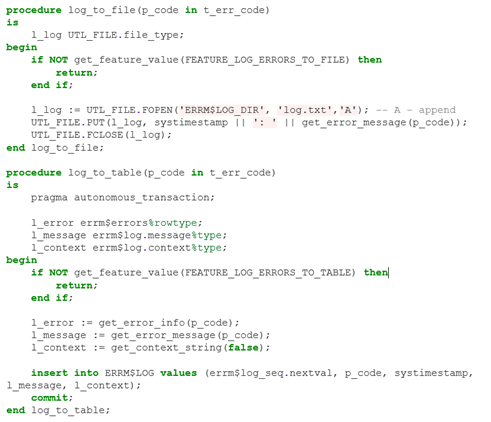
\includegraphics [scale=1] {my_folder/img/c3_log_to_file_code.png}
	\caption{Коды процедур логирования в файл и в таблицу} 
	\label{fig:c3_log_to_file_code}  
\end{figure}
\FloatBarrier

На \firef{fig:c3_log_to_file_code} представлены процедуры для занесения информации в файл и в таблицу, соответственно. Каждая процедура перед логированием информации, проверяет включена ли соответствующая опция. Метод LOG\_TO\_FILE открывает файл при помощи функции UTL\_FILE.FOPEN, с параметром A, который позволяет добавить информацию в конец файла и заносит необходимую информацию. 

Метод LOG\_TO\_TABLE получает необходимые значения, сюда входит: номер лога, сообщение об ошибке, контекст ошибки, а затем вносит данные в таблицу. Метод объявлен как автономная транзакция, это необходимо для того, чтобы данные в таблице ERRM\$LOG не откатились вместе с основной транзакцией при возникновении ошибки (которая будет далее вызвана методом RAISE).

\begin{figure}[ht!] 
	\center
	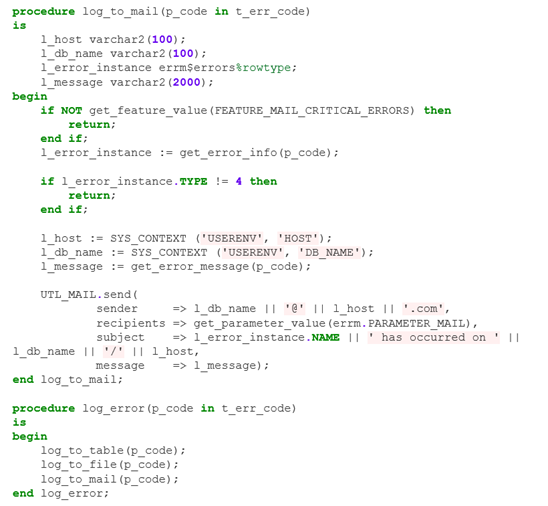
\includegraphics [scale=1] {my_folder/img/c3_log_code.png}
	\caption{Код логирования ошибок} 
	\label{fig:c3_log_code}  
\end{figure}
\FloatBarrier

Код, представленный на \firef{fig:c3_log_code} отвечает за логирование критических ошибок на почту, и общий метод логирования, который и вызывает процедура RAISE. Процедура LOG\_TO\_MAIL, отправляет письмо администратору, адрес которого указывается в параметрах приложения. 

Процедура LOG\_ERROR по очереди вызывает ранее описанные методы. 

Очистка мест сбора информации происходит следующим образом. В случае хранения информации в файле (метод CLEAR\_LOG\_FILE), файл открывается для записи, при помощи пакета UTL\_FILES, функцией FOPEN, с указанием параметра W, что очистит файл для записи новой информации. После чего файл сразу же закрывается. В результате данного действия файл станет пустым. 

Сложнее происходит очистка таблицы ERRM\$LOG, помимо удаления данных из самой таблицы, необходимо обнулить последовательность номеров лога. Пересоздать последовательность заново мы не можем, так как, в этом случае пакет (имеющий зависимость на эту последовательность) потребует перекомпиляции. Обнулять последовательность будем способом, показанным на \firef{fig:c3_clear_code}. 

\begin{figure}[ht!] 
	\center
	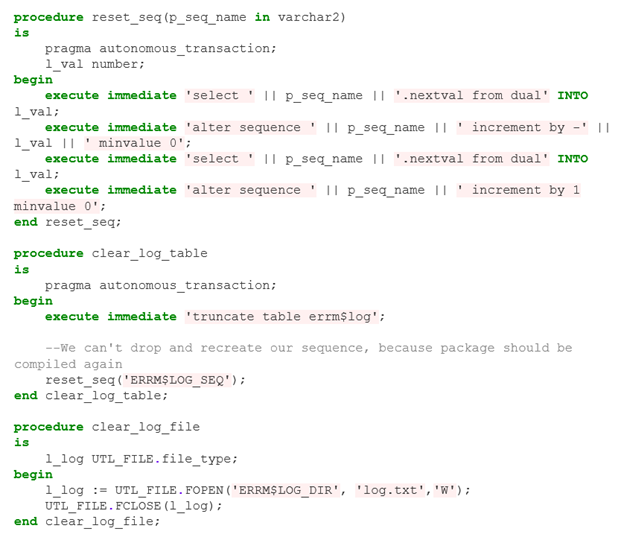
\includegraphics [scale=1] {my_folder/img/c3_clear_code.png}
	\caption{Код процедур для очистки мест логирования} 
	\label{fig:c3_clear_code}  
\end{figure}
\FloatBarrier

Здесь представлен фрагмент кода с очисткой файла логирования, и метод для очистки таблицы логирования. Сама очистка таблицы происходит посредством вызова динамического SQL кода, а конкретно команды TRUNCATE TABLE, после чего происходит вызов процедуры RESET\_SEQ, в который передается имя последовательности. 
В методе RESET\_SEQ происходит динамический вызов четырех команд SQL. Первоначально из последовательности извлекается следующее число, далее происходит изменение последовательности при помощи команды ALTER SEQUENCE, изменяется шаг на отрицательное значение, полученного на прошлом этапе числа. Далее извлекается следующее значение последовательности, в результате чего текущее число последовательности обнулится. Последняя команда возвращает шаг последовательности к начальному значению. 


\section{Работа с контекстом} \label{ch3:sec8}

Для сохранения контекста ошибки будет использоваться схема, описанная далее. В теле пакета объявляется тип данных t\_context, являющийся таблицей, хранящей тип varchar2 и индексируемой типом varchar2 (аналог ассоциативного массива в PL/SQL, еще называемый словарем). А также объект данного типа с именем g\_context. При помощи метода ADD\_CONTEXT, в данный словарь будут вноситься данные. При возникновении ошибки информация из контекста попадает в лог, ассоциативный массив очищается, для хранения контекста новых ошибок. Процедура CLEAR\_CONTEXT позволяет очищать контекст вручную, в случае необходимости. 
Дополнительная процедура ADD\_DEFAULT\_CONTEXT добавляет к контексту системную информацию, в нее включены: наименование экземпляра, обслуживающего базу, наименование базы данных, имя пользователя, имя приложения из которого выполнялась работа, текущая схема, наименование хоста. Описанный базовый контекст может добавляться автоматически, ко всем возникшим ошибкам, это поведение настраивается флагом в таблице ERRM\$FEATURE\_FLAGS, по умолчанию включено.  

\begin{figure}[ht!] 
	\center
	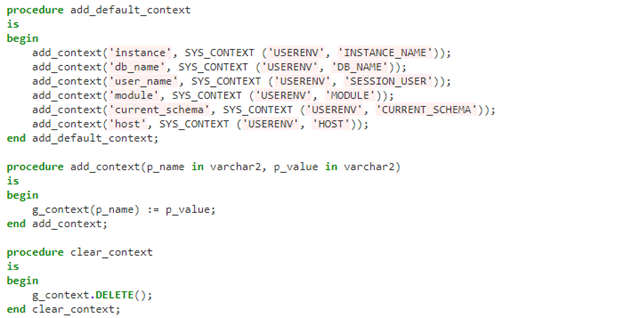
\includegraphics [scale=1] {my_folder/img/c3_add_context_code.png}
	\caption{Методы добавления информации в контекст ошибки} 
	\label{fig:c3_add_context_code}  
\end{figure}
\FloatBarrier

На фрагменте кода, представленном на \firef{fig:c3_add_context_code}, показаны методы для добавления контекста, для очистки словаря контекста, и для заполнения словаря контекстом по умолчанию. 

Так же для работы с контекстом, используется метод GET\_CONTEXT\_STRING, который формирует из словаря строку с информацией о хранящихся в контексте данных, которая в дальнейшем добавляется в лог. Код данной функции представлен на \firef{fig:c3_get_context_code}.


\begin{figure}[ht!] 
	\center
	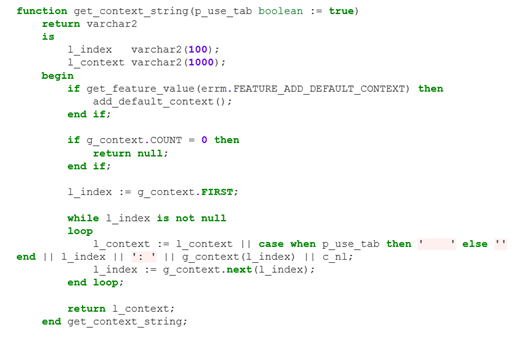
\includegraphics [scale=1] {my_folder/img/c3_get_context_code.png}
	\caption{Функция получения строки контекста} 
	\label{fig:c3_get_context_code}  
\end{figure}
\FloatBarrier

Добавление контекста по умолчанию, происходит именно в этом методе, так как строка с контекстом обязательно будет запрошено при вызове исключения. В качестве параметра, данная функция принимает флаг, указывающий нужно добавлять дополнительный отступ перед параметрами контекста, для логирования в таблицу данный отступ не является необходимым, потому что контекст будет храниться в отдельном столбце, а для вывода на экран и в файл, отступ будет упрощать чтение сообщения об ошибке.

Данный подход для работы с контекстом почти не ограничивает пользователя в хранимом количестве данных, ограничение появляется только при достижении лимита размера типа varchar2. Максимальный размер данного типа 4000 байт, что эквивалентно 4000 символов в одно байтовой кодировке или 2000 символов в двухбайтовой. Данного объема обычно достаточно для ошибок, контекст ошибки не должен содержать больших данных, но при этом должен давать максимально подробное описание ситуации. В дальнейшем, при необходимости, можно реализовать альтернативный механизм хранения контекста, который не подвержен данному ограничению, например, большой контекст помещать в файл, а в основном контексте оставлять ссылку на файл. 

\section{Отчеты об ошибках} \label{ch3:sec9}
 
Были создали два представления для получения информации о популярных ошибках и о самых часто встречающихся. 

\begin{figure}[ht!] 
	\center
	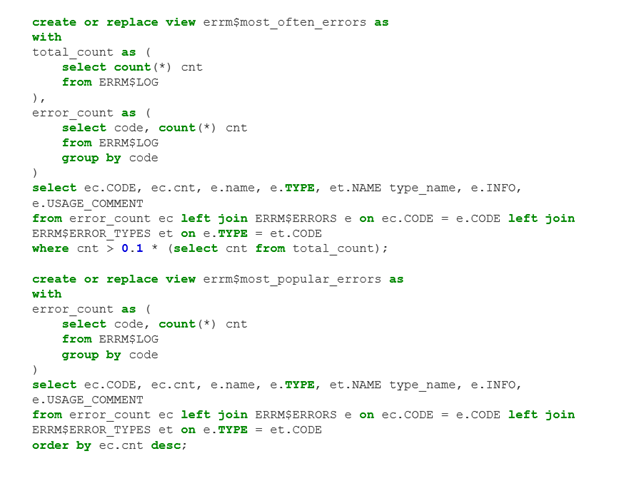
\includegraphics [scale=1] {my_folder/img/c3_view_code.png}
	\caption{Создание представлений} 
	\label{fig:c3_view_code}  
\end{figure}
\FloatBarrier

Код на \firef{fig:c3_view_code}, показывает, как создаются указанные представления. 
В представлении ERRM\$MOST\_OFTEN\_ERRORS содержится информация о тех ошибках, что встречаются чаще 10\% от общего числа сохраненных ошибок. 
Представление ERRM\$MOST\_POPULAR\_ERRORS содержит список всех возникших ошибок, отсортированный по количеству появлений. 


\section{Удаление пакета} \label{ch3:sec10}

Для удаления пакета из системы был разработан скрипт, в котором реализована правильная последовательность удаления объектов пакета. 

\begin{figure}[ht!] 
	\center
	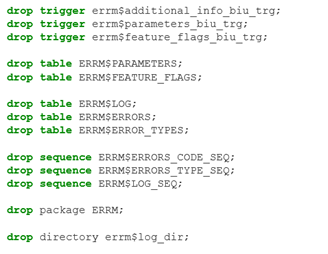
\includegraphics [scale=1] {my_folder/img/c3_uninstall.png}
	\caption{Скрипт удаления пакета} 
	\label{fig:c3_uninstall}  
\end{figure}
\FloatBarrier

На \firef{fig:c3_uninstall} представлен данный скрипт. В первую очередь удалим триггеры. Далее необходимо удалить объекты в обратной последовательности от их создания. Сначала удаляются таблицы, не имеющие зависимостей, затем происходит удаление таблиц, на которые не ссылаются другие таблицы (изначально существует только одна такая таблица это ERRM\$LOG, поэтому она удаляется первой, затем таблица ERRM\$ERRORS не имеет таблиц, ссылающихся на нее, и может быть удалена), и далее по цепочке. Затем удаляются созданные во время установки последовательности. В последнюю очередь удаляется сам пакет и директория для логирования.
Полный код пакета, и всех остальных скриптов можно посмотреть в приложении \ref{appendix-1}. 


\section{Выводы} \label{ch3:conclusion}


В данной главе был разработан пакет для работы с ошибками, были созданы скрипты для установки и удаления данного пакета, разобраны основные методы пакета. Рассмотрены алгоритмы сохранения информации об ошибках. 


%% Вспомогательные команды - Additional commands
%
\newpage % принудительное начало с новой страницы, использовать только в конце раздела
%\clearpage % осуществляется пакетом <<placeins>> в пределах секций
%\newpage\leavevmode\thispagestyle{empty}\newpage % 100 % начало новой страницы           	 % Глава 3
\chapter{Тестирование и апробация пакета} \label{ch4}

% не рекомендуется использовать отдельную section <<введение>> после лета 2020 года
%\section{Введение} \label{ch4:intro}

В данной главе описываются используемые методы проверки корректности работы различных аспектов разработанного пакета. Далее в параграфе \ref{ch4:sec4} проводится сравнение использования пакета для работы с ошибками со стандартным методом, предлагаемым Oracle. 
	
\section{Проверка установки пакета} \label{ch4:sec}

В первую очередь была написана инструкция по установке и удалению, и помещена к инсталлеру. После чего был протестирован скрипт создания пакета и его удаления. Замеченные недостатки устранялись, на данном этапе была поправлена последовательность создания и удаления объектов. Проверялась правильность очистки базы, после удаления пакета, корректной работой считается полное отсутствие объектов, принадлежащих пакету. Была проверена установка значений параметров по умолчанию, в ходе тестирования были модифицированы некоторые значения параметров, для максимального быстродействия. 

\section{Проверка работы пакета} \label{ch4:sec2}

Для тестирования пакета был написан скрипт, содержащий тестовые случаи, который был добавлен к скрипту установщику. Была проверена работа всех, объявленных в спецификации пакета, процедур и функций в различных ситуациях и с разными настройками пакета. Рассматривались как положительные случаи, так и отрицательные ситуации (некорректные данные, отсутствующие данные). Часть тестов была автоматизирована, часть оставлена для ручной проверки. Автоматические тесты выполняют несколько ситуаций и сравнивают результат с эталоном, после чего выводят на экран результат проверки. 

На \firef{fig:c4_auto_test} представлена часть кода автоматических тестов. 

\begin{figure}[ht!] 
	\center
	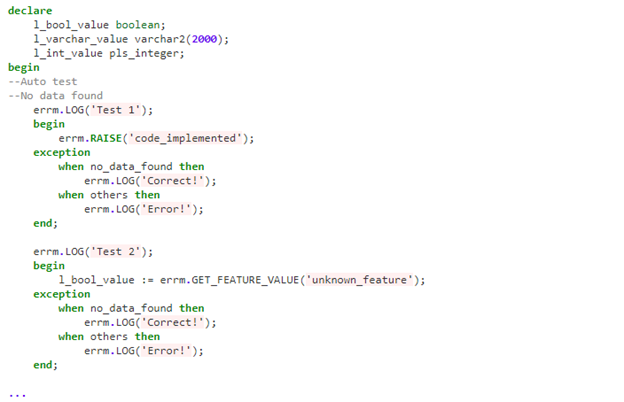
\includegraphics [scale=1] {my_folder/img/c4_auto_test.png}
	\caption{Пример кода автоматических тестов} 
	\label{fig:c4_auto_test}  
\end{figure}
\FloatBarrier

Первый тест проверяет вызов несуществующий ошибки по ее имени. Второй, пытается получить значение опции, по имени, которое не содержится в таблице ERRM\$FEATURE\_FLAGS. 

Остальные автоматические тесты проверяют следующие ситуации.

Тест 3 устанавливает значение несуществующей опции.

Тест 4 устанавливает значение параметра, которого не существует.

Тест 5 пытается получить значение отсутствующего параметра.

В тесте 6 проверяется ситуация получения кода ошибки, которая не определена.

Вызов ошибки с несуществующим кодом проводится в тесте 7.

Тест 8 повторяет 7 тест, но запрещает логирование.

Тест 9 вызывает ошибку по имени, которой не существует.

Тест 10 делает тоже самое, но без логирования.

Тесты 11 и 12 проверяют методы SRAISE с кодом и именем не существующих ошибок, соответственно. 
Каждый тест обернут в блок begin/end с обработчиком ошибки, если возникла правильная ошибка, тест возвращает корректный результат, если возникла другая ошибка, тест сообщает о неудаче. 

9 ручных тестов предназначены для проверки корректности работы основных методов, а также некоторых параметров и опций пакета.

\begin{figure}[ht!] 
	\center
	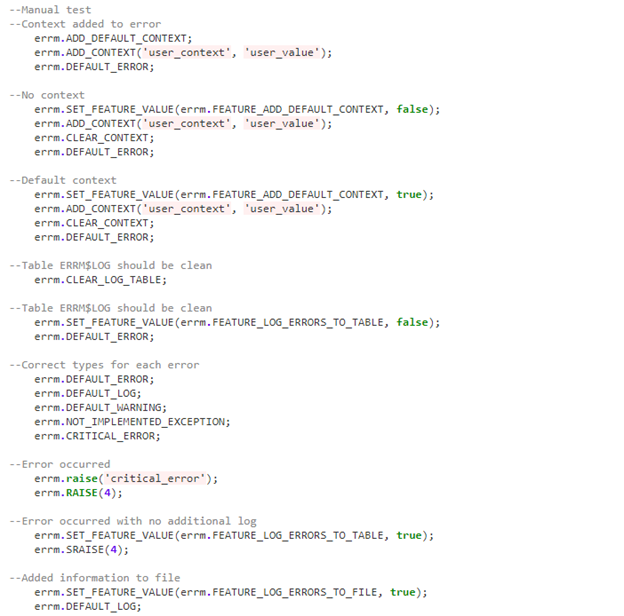
\includegraphics [scale=1] {my_folder/img/c4_manual_test.png}
	\caption{Код для ручного тестирования пакета} 
	\label{fig:c4_manual_test}  
\end{figure}
\FloatBarrier

На \firef{fig:c4_manual_test} представлены ручные тесты. Каждый случай содержит комментарий с описанием ожидаемого результата.

Первая ситуация проверяет добавление контекста к ошибке.
 
Второй тест проверяет возможность очистки контекста. 

Третий тест демонстрирует как должна работать очистка контекста, в ситуации с автоматическим добавлением стандартного контекста. 

Четвертый тест проверяет корректность очистки таблицы логирования.

Тест под номер пять проверяет флаг для отключения логирования в таблицу. 

Тест 6 состоит из вызова нескольких предопределенных ошибок, здесь проверяется корректность типов ошибок, и в целом работа всей системы.

Тест 7 проверяет вызов ошибки по имени и коду.

Тест 8 проверяет корректность работы методов «тихого» вызова исключения. 

Тест 9 проверяет запись в файл логирования. 

Помимо этого, была проверена запись логов в файл, корректность отработки внутренних (скрытых от пользователя в теле пакета) методов, были проверены ситуации добавления значений в контекст с одинаковым ключом, множественное добавление базового контекста и некоторые другие случаи.

Все найденные в ходе тестирования ошибки и недочеты исправлялись. 

Не удалось настроить работу почтового сервиса на виртуальной машине, поэтому тестирование отправки Email сообщение провалилось. Данная опция была отключена по умолчанию. 

\section{Улучшение кода} \label{ch4:sec3}

Во время проверки составлялся список субъективных ощущений от работы с пакетом, после чего данный список был проанализирован, неудобства в работе с пакетом скорректированы. 

Был проведен рефакторинг с целью улучшения работы пакета. В ходе него были удалены неиспользуемые переменные и методы, были устранены некоторые узкие места, были пересмотрены используемые типы данных, и сигнатуры некоторых методов.

После рефакторинга было проведено дополнительно полное тестирование пакета, с целью выявление регресса. Найденные проблемы были устранены. 


\section{Сравнение полученных результатов} \label{ch4:sec4}

На \firef{fig:c4_examples} представлены три примера кода, работающего с исключительными ситуациями. 

\begin{figure}[ht!] 
	\center
	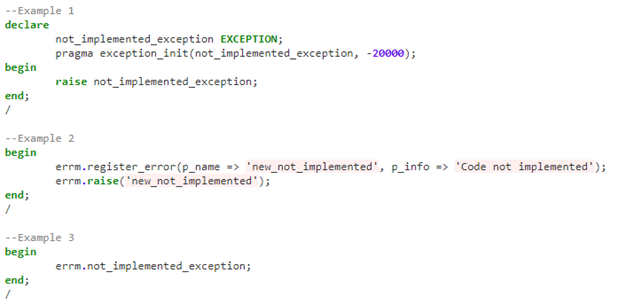
\includegraphics [scale=1] {my_folder/img/c4_examples.png}
	\caption{Примеры использования пакета} 
	\label{fig:c4_examples}  
\end{figure}
\FloatBarrier

Пример 1 использует стандартные средства для вызова исключения. Пример 2 объявляет новое исключение при помощи пакета, а затем вызывает его. Пример 3 вызывает существующее исключение. 

Второй код больше приближен к первому примеру, так как создается новое исключение, и выигрыш в объеме кода является не таким значимым, первый случай содержит 150 символов, в то время как во второй ситуации только 136, но второй пример имеет значительный выигрыш в других показателях. 

Результаты выполнения первого примера показаны на \firef{fig:c4_1_example_res}:

\begin{figure}[ht!] 
	\center
	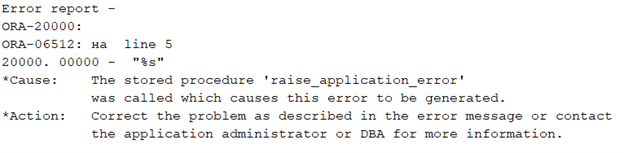
\includegraphics [scale=1] {my_folder/img/c4_1_example_res.png}
	\caption{Результаты выполнения первого примера} 
	\label{fig:c4_1_example_res}  
\end{figure}
\FloatBarrier

На \firef{fig:c4_2_example_res} представлены результаты выполнения второго кода:

\begin{figure}[ht!] 
	\center
	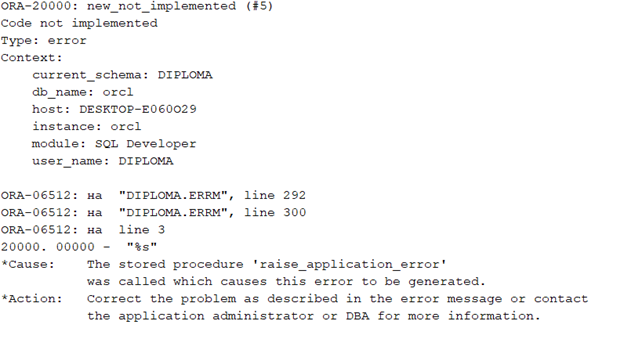
\includegraphics [scale=1] {my_folder/img/c4_2_example_res.png}
	\caption{Результаты выполнения второго примера} 
	\label{fig:c4_2_example_res}  
\end{figure}
\FloatBarrier

В первом случае мы не получили никакой информации об ошибке, сообщение пустое, почему возникло исключение в коде не понятно. В то время второй код, содержит описание о возникшей ошибке (которая только что создана), а также дополнительную мета информацию, помимо этого, сообщение об ошибке будет занесено в таблицу логирования, и в файл логов. Созданная ошибка сразу будет видна другим исполняемым блокам, в то же время информация об ошибке в первом примере доступна только самому анонимному блоку и его вложенным блокам. 

Созданную ошибку можно заново использовать без дополнительного кода. Нет необходимости следить за кодами ошибок. Информацию обо всех существующих ошибках можно легко узнать из одной таблицы ERRM\$ERRORS. 

Пример под номером три, показывает работу пакета в ситуации более приближенной к реальной разработке, обычно мы хотим использовать уже известную исключительную ситуацию, для часто используемых ошибок, достаточно вызвать единственный метод без параметров. При этом мы получим результат подобный примеру 2, и соответственно все его преимущества. Третий пример состоит всего из 44 символов, следовательно мы потратим меньше времени на написание кода, а важнее то, что нам не потребуется выполнять дополнительные действия для простых ситуаций. 

Следующий пример, представленный на рисунке \firef{fig:c4_add_context_example}, демонстрирует использование контекста для сохранения значений параметров.

\begin{figure}[ht!] 
	\center
	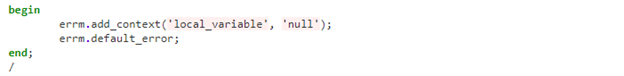
\includegraphics [scale=1] {my_folder/img/c4_add_context_example.png}
	\caption{Пример добавления контекста} 
	\label{fig:c4_add_context_example}  
\end{figure}
\FloatBarrier

В результате выполнения этого скрипта, в сообщение об ошибке (а также во всех местах куда логируется информация, согласно настройкам) будет содержаться указанная нами информация, что в перспективе облегчит отладку, и исправление ошибки. 

Указанные выше примеры, а также некоторые дополнительные, были объединены в один скрипт, который будет распространяться вместе с пакетом для демонстрации различных возможностей приложения.



\section{Выводы} \label{ch4:conclusion}

В данной главе было проведено тестирование кода, а также его улучшение и настройка. Были приведены примеры работы с пакетом, а также сравнение разработанного пакета в работе со стандартным способом. 
           	 % Глава 3
\ContinueChapterEnd % завершить размещение глав <<подряд>>
%% Завершение основной части

\chapter*{Заключение} \label{ch-conclusion}
\addcontentsline{toc}{chapter}{Заключение}	% в оглавление 

В данной работе были изучены механизмы взаимодействия с исключительными ситуациями, предоставляемые разработчикам приложений в базе данных Oracle на языке PL/SQL. В ходе изучения данной систем были выявлены некоторые недостатки и неудобства, усложняющие процесс создания новых приложений. Основной проблемой являлось необходимость дополнительных действий со стороны команды программистов для контроля над исключительными ситуациями. Возможность упростить данный процесс, послужила поводом для разработки пакета.
 
Были рассмотрены различные способы устранения большинства критических проблем. Из предложенных решений были выбраны самые оптимальные и наиболее эффективные алгоритмы. На основе данных алгоритмов был разработан пакет на языке PL/SQL. Используемые подходы были подробно рассмотрены, была описана обоснованность и целесообразность их использования. Пакет был разработан с обширными возможностями для его дальнейшего расширения, как со стороны автора, так и со стороны пользователей пакета. 

Полученный пакет был тщательно протестирован на выявление ошибок при работе. Тестированию подлежали все элементы пакета, начиная с публичных методов, доступных пользователю, заканчивая скрытыми методами, которые необходимы для выполнения внутренних задач.
 
Данное решение подверглось сравнению со стандартным способом обработки исключительных ситуаций, предоставляемым разработчикам кампанией Oracle. Был выявлен ряд существенных упрощений при разработке с использованием созданного пакета. 


        	 % Заключение

%% Наличие следующих перечней не исключает расшифровку сокращения и условного обозначения при первом упоминании в тексте!
%%\input{my_folder/acronyms}		         % Необязательная рубрика! Список сокращений и условных обозначений

%%\input{my_folder/dictionary}    		 % Необязательная рубрика! Словарь терминов
% По порядку после Списка сокращений и условных обозначений, если есть.	


\input{my_folder/references}		     % Список литературы

% Здесь можно поместить список иллюстративного материала

\appendix % не редактировать / keep unmodified


\chapter{Код пакета}\label{appendix-1}							% Заголовок
%\addcontentsline{toc}{chapter}{Second call for chapters to participate in the book Machine learning in analysis of biomedical and socio-economic data}	% Добавляем его в оглавление
\section{Код установочного скрипта}\label{app-1}
Файл install\_script.sql:

%\begin{lstlisting}
\begin{verbatim}
--CREATE ERROR_TYPES TABLE
create table errm$error_types (
code number(5) primary key,
name varchar2(100 char) unique not null,
info varchar2(2000 char)
);

create sequence errm$errors_type_seq start with 4 increment by 1;

insert into errm$error_types values (0, 'error', 'Exception');
insert into errm$error_types values (1, 'warning', 'Warning');
insert into errm$error_types values (2, 'log', 'Log information');
insert into errm$error_types values (3, 'critical_error', 'Exceptions that require additional actions');

--CREATE ERRORS TABLE
create table errm$errors (
code number(10) primary key,
name varchar2(100) unique not null,
type number(5) default 0 references errm$error_types not null,
info varchar2(2000) not null,
usage_comment varchar2(1000),
create_date date,
create_by varchar2(100)
);
/

create sequence errm$errors_code_seq start with 5 increment by 1;

create or replace trigger errm$additional_info_biu_trg
before insert or update
on errm$errors
for each row
begin
:new.name := lower(:new.name);
if :old.create_date is null then
:new.create_date := sysdate;
:new.create_by := SYS_CONTEXT ('USERENV', 'SESSION_USER');
end if;
end errm$additional_info_biu_trg;

insert into errm$errors values (0, 'default_error', 0, 'Error has occurred', 'Simple error for tests. Do not use it in production!', null, null);
insert into errm$errors values (1, 'not_implemented', 0, 'Code not implemented', 'Use when code not yet implemented.', null, null);
insert into errm$errors values (2, 'default_warning', 1, 'Warning information', 'Simple warning for tests. Do not use it in production!', null, null);
insert into errm$errors values (3, 'default_log', 2, 'Log information', 'Simple log message for tests. Do not use it in production!', null, null);
insert into errm$errors values (4, 'critical_error', 3, 'Critical error has occurred', 'Simple critical error for tests. Do not use it in production!', null, null);

--CREATE LOG TABLE
create table errm$log (
id number(38) primary key,
code number(10) references errm$errors not null,
timestamp timestamp not null,
message varchar2(1000),
context varchar2(2000)
);

create sequence errm$log_seq start with 1 increment by 1;

create table errm$parameters (
name varchar2(50) primary key,
value varchar2(1000)
);

insert into errm$parameters values ('MAIL', 'mikl181@yandex.ru');

create or replace trigger errm$parameters_biu_trg
before insert or update
on errm$parameters
for each row
begin
:NEW.name := upper(:NEW.name);
:NEW.value := lower(:NEW.value);
end errm$parameters_biu_trg;

create table errm$feature_flags (
name varchar2(50) primary key,
value char(1) default '0'
);

insert into errm$feature_flags values ('ALWAYS_ADD_DEFAULT_CONTEXT', '1');
insert into errm$feature_flags values ('MAIL_CRITICAL_ERRORS', '0');
insert into errm$feature_flags values ('LOG_ERRORS_TO_FILE', '1');
insert into errm$feature_flags values ('LOG_ERRORS_TO_TABLE', '1');

create or replace trigger errm$feature_flags_biu_trg
before insert or update
on errm$feature_flags
for each row
begin
:NEW.name := upper(:NEW.name);

if (:new.value not in ('0', '1')) then
raise_application_error(-20000, 'Invalid data');
end if;
end errm$feature_flags_biu_trg;

create or replace view errm$most_often_errors as
with
total_count as (
select count(*) cnt
from ERRM$LOG
),
error_count as (
select code, count(*) cnt
from ERRM$LOG
group by code
)
select ec.CODE, ec.cnt, e.name, e.TYPE, et.NAME type_name, e.INFO, e.USAGE_COMMENT
from error_count ec left join ERRM$ERRORS e on ec.CODE = e.CODE left join ERRM$ERROR_TYPES et on e.TYPE = et.CODE
where cnt > 0.1 * (select cnt from total_count);

create or replace view errm$most_popular_errors as
with
error_count as (
select code, count(*) cnt
from ERRM$LOG
group by code
)
select ec.CODE, ec.cnt, e.name, e.TYPE, et.NAME type_name, e.INFO, e.USAGE_COMMENT
from error_count ec left join ERRM$ERRORS e on ec.CODE = e.CODE left join ERRM$ERROR_TYPES et on e.TYPE = et.CODE
order by ec.cnt desc;

create directory errm$log_dir as 'E:/ERRM';

@@errm.pks
@@errm.pkb
\end{verbatim}


\section{Код спецификации пакета}\label{app-2}
Файл errm.pks:

\begin{verbatim}
create or replace package errm
is
--CONSTANTS
feature_mail_critical_errors constant varchar2(50 char) := 'MAIL_CRITICAL_ERRORS';
feature_log_errors_to_file constant varchar2(50 char) := 'LOG_ERRORS_TO_FILE';
feature_log_errors_to_table constant varchar2(50 char) := 'LOG_ERRORS_TO_TABLE';
feature_add_default_context constant varchar2(50 char) := 'ALWAYS_ADD_DEFAULT_CONTEXT';

parameter_mail constant varchar2(50 char) := 'MAIL';

--TYPES
subtype t_err_code is pls_integer;
subtype t_err_name is varchar2(100 char);
subtype t_err_type is pls_integer;

--PARAMETERS WORK
function get_feature_value(p_feature_name in varchar2) return boolean;
procedure set_feature_value(p_feature_name in varchar2, p_value in BOOLEAN);

function get_parameter_value(p_param_name in varchar2) return varchar2;
procedure set_parameter_value(p_param_name in varchar2, p_value in varchar2);

--HELPERS
function get_error_code(p_name in t_err_name) return t_err_code;

--PROCEDURE AND FUNCTIONS
procedure register_error(p_code in t_err_code := null, p_name in t_err_name, p_type t_err_type := 0, p_info in varchar2, p_comment in varchar2 := null);

procedure add_default_context;
procedure add_context(p_name in varchar2, p_value in varchar2);
procedure clear_context;

procedure raise(p_code in t_err_code, p_log_enabled in boolean := TRUE);
procedure raise(p_name in t_err_name, p_log_enabled in boolean := TRUE);

--SILENT RAISES
procedure sraise(p_code in t_err_code);
procedure sraise(p_name in t_err_name);

--LOG WORK
procedure clear_log_table;
procedure clear_log_file;

--SIMPLE ERRORS RAISE
procedure default_error;
procedure default_log;
procedure default_warning;
procedure critical_error;
procedure not_implemented_exception;

--LOG
procedure log (p_text in varchar2);
procedure nl;
end errm;
/
\end{verbatim}

\section{Код тела пакета}\label{app-3}
Файл errm.pkb:

\begin{verbatim}
create or replace package body errm
is
--CONSTANTS

c_default_error constant pls_integer := -20000;
--New line symbol
c_nl constant char(1) := chr(10);


--TYPES

TYPE t_context IS TABLE OF VARCHAR2(100) INDEX BY VARCHAR2(100);

--VARIABLES

g_context t_context;

--PARAMETERS WORK

function get_feature_value(p_feature_name varchar2)
return boolean
is
l_value errm$feature_flags.value%type;
begin
select value
into l_value
from ERRM$FEATURE_FLAGS
where NAME = upper(p_feature_name);

return l_value = '1';
end get_feature_value;

procedure set_feature_value(p_feature_name varchar2, p_value BOOLEAN)
is
pragma autonomous_transaction;
begin

if p_value then
update ERRM$FEATURE_FLAGS
set value = '1'
where NAME = upper(p_feature_name);
else
update ERRM$FEATURE_FLAGS
set value = '0'
where NAME = upper(p_feature_name);
end if;

if sql%rowcount = 0 then
raise no_data_found;
end if;
commit;
end set_feature_value;

function get_parameter_value(p_param_name varchar2)
return varchar2
is
l_value ERRM$PARAMETERS.value%type;
begin
select value
into l_value
from ERRM$PARAMETERS
where NAME = upper(p_param_name);

return l_value;
end get_parameter_value;

procedure set_parameter_value(p_param_name varchar2, p_value varchar2)
is
pragma autonomous_transaction;
begin
update ERRM$PARAMETERS
set value = lower(p_value)
where NAME = upper(p_param_name);

if sql%rowcount = 0 then
raise no_data_found;
end if;
commit;
end set_parameter_value;


--HELPERS

procedure reset_seq(p_seq_name in varchar2)
is
pragma autonomous_transaction;
l_val number;
begin
--Hack from AskTom for reset sequence
execute immediate 'select ' || p_seq_name || '.nextval from dual' INTO l_val;
execute immediate 'alter sequence ' || p_seq_name || ' increment by -' || l_val || ' minvalue 0';
execute immediate 'select ' || p_seq_name || '.nextval from dual' INTO l_val;
execute immediate 'alter sequence ' || p_seq_name || ' increment by 1 minvalue 0';
end reset_seq;

procedure add_default_context
is
begin
add_context('instance', SYS_CONTEXT ('USERENV', 'INSTANCE_NAME'));
add_context('db_name', SYS_CONTEXT ('USERENV', 'DB_NAME'));
add_context('user_name', SYS_CONTEXT ('USERENV', 'SESSION_USER'));
add_context('module', SYS_CONTEXT ('USERENV', 'MODULE'));
add_context('current_schema', SYS_CONTEXT ('USERENV', 'CURRENT_SCHEMA'));
add_context('host', SYS_CONTEXT ('USERENV', 'HOST'));
end add_default_context;

procedure add_context(p_name in varchar2, p_value in varchar2)
is
begin
g_context(p_name) := p_value;
end add_context;

procedure clear_context
is
begin
g_context.DELETE();
end clear_context;

function get_error_info(p_code in t_err_code)
return errm$errors%rowtype
is
l_error errm$errors%rowtype;
begin
select *
into l_error
from ERRM$ERRORS
where code = p_code;

return l_error;
end get_error_info;

function get_context_string(p_use_tab boolean := true)
return varchar2
is
l_index   varchar2(100);
l_context varchar2(1000);
begin
if get_feature_value(errm.FEATURE_ADD_DEFAULT_CONTEXT) then
add_default_context();
end if;

if g_context.COUNT = 0 then
return null;
end if;

l_index := g_context.FIRST;

while l_index is not null
loop
l_context := l_context || case when p_use_tab then '    ' else '' end || l_index || ': ' || g_context(l_index) || c_nl;
l_index := g_context.next(l_index);
end loop;

return l_context;
end get_context_string;

function get_error_message(p_code in t_err_code)
return varchar2
is
r_error_instance errm$errors%rowtype;
l_error_typename errm$error_types.name%type;
l_context varchar2(2000);
begin
r_error_instance := get_error_info(p_code);

select name
into l_error_typename
from ERRM$ERROR_TYPES
where code = r_error_instance.TYPE;

l_context := get_context_string();

return  r_error_instance.name || ' (#' || p_code ||')' || c_nl ||
r_error_instance.info || c_nl ||
'Type: ' || l_error_typename || c_nl ||
'Context' ||
case
when l_context is null then
' not provided!'
else
': ' || c_nl || l_context
end
|| c_nl;
end get_error_message;


procedure log_to_file(p_code in t_err_code)
is
l_log UTL_FILE.file_type;
begin
if NOT get_feature_value(FEATURE_LOG_ERRORS_TO_FILE) then
return;
end if;

l_log := UTL_FILE.FOPEN('ERRM$LOG_DIR', 'log.txt','A'); -- A - append
UTL_FILE.PUT(l_log, systimestamp || ': ' || get_error_message(p_code));
UTL_FILE.FCLOSE(l_log);
end log_to_file;

procedure log_to_table(p_code in t_err_code)
is
pragma autonomous_transaction;

l_error errm$errors%rowtype;
l_message errm$log.message%type;
l_context errm$log.context%type;
begin
if NOT get_feature_value(FEATURE_LOG_ERRORS_TO_TABLE) then
return;
end if;

l_error := get_error_info(p_code);
l_message := get_error_message(p_code);
l_context := get_context_string(false);

insert into ERRM$LOG values (errm$log_seq.nextval, p_code, systimestamp, l_message, l_context);
commit;
end log_to_table;

procedure log_to_mail(p_code in t_err_code)
is
l_host varchar2(100);
l_db_name varchar2(100);
l_error_instance errm$errors%rowtype;
l_message varchar2(2000);
begin
if NOT get_feature_value(FEATURE_MAIL_CRITICAL_ERRORS) then
return;
end if;
l_error_instance := get_error_info(p_code);

if l_error_instance.TYPE != 4 then
return;
end if;

l_host := SYS_CONTEXT ('USERENV', 'HOST');
l_db_name := SYS_CONTEXT ('USERENV', 'DB_NAME');
l_message := get_error_message(p_code);

UTL_MAIL.send(
sender     => l_db_name || '@' || l_host || '.com',
recipients => get_parameter_value(errm.PARAMETER_MAIL),
subject    => l_error_instance.NAME || ' has occurred on ' || l_db_name || '/' || l_host,
message    => l_message);
end log_to_mail;

procedure log_error(p_code in t_err_code)
is
begin
log_to_table(p_code);
log_to_file(p_code);
log_to_mail(p_code);
end log_error;

function get_error_code(p_name in t_err_name)
return t_err_code
is
l_err_code t_err_code;
begin
select code
into l_err_code
from errm$errors
where lower(name) = lower(p_name);

return l_err_code;
end get_error_code;


--PROCEDURE AND FUNCTIONS

procedure register_error(p_code in t_err_code := null, p_name in t_err_name, p_type t_err_type := 0, p_info in varchar2, p_comment in varchar2)
is
pragma autonomous_transaction;
begin
insert into ERRM$ERRORS
values (NVL(p_code, errm$errors_code_seq.nextval), lower(p_name), p_type, p_info, p_comment, null, null);
commit;
end register_error;


procedure raise(p_code in t_err_code, p_log_enabled in boolean := TRUE)
is
l_message varchar2(2000);
begin
if p_log_enabled then
log_error(p_code);
end if;

l_message := get_error_message(p_code);

clear_context();
raise_application_error(c_default_error, l_message);
end raise;

procedure raise(p_name in t_err_name, p_log_enabled in boolean := TRUE)
is
l_err_code t_err_code;
begin
l_err_code := get_error_code(p_name);
errm.raise(l_err_code, p_log_enabled);
end raise;

procedure sraise(p_code in t_err_code)
is
begin
errm.raise(p_code, FALSE);
end sraise;

procedure sraise(p_name in t_err_name)
is
begin
errm.raise(p_name, FALSE);
end sraise;


--LOG WORK

procedure clear_log_table
is
pragma autonomous_transaction;
begin
execute immediate 'truncate table errm$log';

--We can't drop and recreate our sequence, because package should be compiled again
reset_seq('ERRM$LOG_SEQ');
end clear_log_table;

procedure clear_log_file
is
l_log UTL_FILE.file_type;
begin
l_log := UTL_FILE.FOPEN('ERRM$LOG_DIR', 'log.txt','W');
UTL_FILE.FCLOSE(l_log);
end clear_log_file;

--EASE ERRORS RAISE

procedure default_error
is
begin
errm.raise(0);
end default_error;

procedure not_implemented_exception
is
begin
errm.raise(1);
end not_implemented_exception;

procedure default_warning
is
begin
errm.raise(2);
end default_warning;

procedure default_log
is
begin
errm.raise(3);
end default_log;

procedure critical_error
is
begin
errm.raise(4);
end critical_error;


--LOG

procedure log (p_text in varchar2)
is
begin
dbms_output.put_line(p_text);
end log;

procedure nl
is
begin
dbms_output.new_line;
end nl;
end errm;
/	
\end{verbatim}

\section{Код скрипта для удаления}\label{app-4}
Файл uninstall.sql:

\begin{verbatim}
drop view ERRM$MOST_OFTEN_ERRORS;
drop view ERRM$MOST_POPULAR_ERRORS;

drop trigger errm$additional_info_biu_trg;
drop trigger errm$parameters_biu_trg;
drop trigger errm$feature_flags_biu_trg;

drop table ERRM$PARAMETERS;
drop table ERRM$FEATURE_FLAGS;

drop table ERRM$LOG;
drop table ERRM$ERRORS;
drop table ERRM$ERROR_TYPES;

drop sequence ERRM$ERRORS_CODE_SEQ;
drop sequence ERRM$ERRORS_TYPE_SEQ;
drop sequence ERRM$LOG_SEQ;

drop package ERRM;

drop directory errm$log_dir;
\end{verbatim}

\section{Файл с инструкциями по установке}\label{app-5}
Файл readme.txt:

\begin{verbatim}
Инструкция по установке пакета.
1. Найти в файле install.sql строку
create directory errm$log_dir as 'E:/ERRM';
2. Заменить путь директории на необходимый для хранения фалйов логирования
3. Настроить пакет UTL_MAIL
4. Выполнить скрипт install.sql
5. Прочитать описание параметров и опций
6. Настроить пакет по своему усмотрению при помощи процедур SET_PARAMETER_VALUE и SET_FEATURE_VALUE

Удаление пакета:
1. Запустить скрипт uninstall.sql
\end{verbatim}

\section{Скрипт с примерами использования пакета}\label{app-6}
Файл examples.sql:

\begin{verbatim}
--Example 1. Standard exception raise
declare
not_implemented_exception EXCEPTION;
pragma exception_init(not_implemented_exception, -20000);
begin
raise not_implemented_exception;
end;
/

--Example 2. Define new error and raise
begin
errm.register_error(p_name => 'new_not_implemented', p_info => 'Code not implemented');
errm.raise('new_not_implemented');
end;
/

--Example 3. Raise predefined error
begin
errm.not_implemented_exception;
end;
/

--Example 4. Using context for save information
begin
errm.add_context('local_variable', 'null');
errm.default_error;
end;
/

--Example 5. Silent raise with code
begin
errm.sraise(1);
end;
/

--Example 6. Silent raise with name
begin
errm.sraise('critical_error');
end;
/

--Example 7. Raise with name
begin
errm.raise('critical_error');
end;
/

--Example 8. Raise with error code
begin
errm.raise(0);
end;
/
\end{verbatim}

\section{Скрипт для тестирования пакета}\label{app-7}
Файл test.sql:

\begin{verbatim}
SET SERVEROUTPUT ON;
declare
l_bool_value boolean;
l_varchar_value varchar2(2000);
l_int_value pls_integer;
begin
--Auto test
--No data found
errm.LOG('Test 1');
begin
errm.RAISE('code_implemented');
exception
when no_data_found then
errm.LOG('Correct!');
when others then
errm.LOG('Error!');
end;

errm.LOG('Test 2');
begin
l_bool_value := errm.GET_FEATURE_VALUE('unknown_feature');
exception
when no_data_found then
errm.LOG('Correct!');
when others then
errm.LOG('Error!');
end;

errm.LOG('Test 3');
begin
errm.SET_FEATURE_VALUE('unknown_feature', false);
exception
when no_data_found then
errm.LOG('Correct!');
when others then
errm.LOG('Error!');
end;

errm.LOG('Test 4');
begin
l_varchar_value := errm.GET_PARAMETER_VALUE('unknown_parameter');
exception
when no_data_found then
errm.LOG('Correct!');
when others then
errm.LOG('Error!');
end;

errm.LOG('Test 5');
begin
errm.SET_PARAMETER_VALUE('unknown_parameter', 'unknown_value');
exception
when no_data_found then
errm.LOG('Correct!');
when others then
errm.LOG('Error!');
end;

errm.LOG('Test 6');
begin
l_int_value := errm.GET_ERROR_CODE('unknown_error');
exception
when no_data_found then
errm.LOG('Correct!');
when others then
errm.LOG('Error!');
end;

errm.LOG('Test 7');
begin
errm.RAISE(-1);
exception
when no_data_found then
errm.LOG('Correct!');
when others then
errm.LOG('Error!');
end;

errm.LOG('Test 8');
begin
errm.RAISE(-1, false);
exception
when no_data_found then
errm.LOG('Correct!');
when others then
errm.LOG('Error!');
end;

errm.LOG('Test 9');
begin
errm.RAISE('unknown_error');
exception
when no_data_found then
errm.LOG('Correct!');
when others then
errm.LOG('Error!');
end;

errm.LOG('Test 10');
begin
errm.RAISE('unknown_error', false);
exception
when no_data_found then
errm.LOG('Correct!');
when others then
errm.LOG('Error!');
end;

errm.LOG('Test 11');
begin
errm.SRAISE(-1);
exception
when no_data_found then
errm.LOG('Correct!');
when others then
errm.LOG('Error!');
end;

errm.LOG('Test 12');
begin
errm.SRAISE('unknown_error');
exception
when no_data_found then
errm.LOG('Correct!');
when others then
errm.LOG('Error!');
end;

--Manual test
--Context added to error
--     errm.ADD_DEFAULT_CONTEXT;
--     errm.ADD_CONTEXT('user_context', 'user_value');
--     errm.DEFAULT_ERROR;

--No context
--     errm.SET_FEATURE_VALUE(errm.FEATURE_ADD_DEFAULT_CONTEXT, false);
--     errm.ADD_CONTEXT('user_context', 'user_value');
--     errm.CLEAR_CONTEXT;
--     errm.DEFAULT_ERROR;

--Default context
--     errm.SET_FEATURE_VALUE(errm.FEATURE_ADD_DEFAULT_CONTEXT, true);
--     errm.ADD_CONTEXT('user_context', 'user_value');
--     errm.CLEAR_CONTEXT;
--     errm.DEFAULT_ERROR;

--Table ERRM$LOG should be clean
--     errm.CLEAR_LOG_TABLE;

--Table ERRM$LOG should be clean
--     errm.SET_FEATURE_VALUE(errm.FEATURE_LOG_ERRORS_TO_TABLE, false);
--     errm.DEFAULT_ERROR;

--Correct types for each error
--     errm.DEFAULT_ERROR;
--     errm.DEFAULT_LOG;
--     errm.DEFAULT_WARNING;
--     errm.NOT_IMPLEMENTED_EXCEPTION;
--     errm.CRITICAL_ERROR;

--Error occurred
--     errm.raise('critical_error');
--     errm.RAISE(4);

--Error occurred with no additional log
--     errm.SET_FEATURE_VALUE(errm.FEATURE_LOG_ERRORS_TO_TABLE, true);
--     errm.SRAISE(4);

--Added information to file
--     errm.SET_FEATURE_VALUE(errm.FEATURE_LOG_ERRORS_TO_FILE, true);
--     errm.DEFAULT_LOG;
end;
/
\end{verbatim}
			     % Приложение 1

%%\input{my_folder/appendix2}			 	 % Приложение 2


\end{document} % конец документа


%%% Удачной защиты ВКР! - Good luck on the thesis defense!
%%
%%% Поддержать проект
%%
%% Запросы на добавление / изменение просим писать на следующей странице:
%% https://github.com/ParkhomenkoV/SPbPU-student-thesis-template/issues
%%
%% Список пожеланий в файле шаблона <<TO-DO-list.tex>>
%%
%% Благодарности просим указывать в виде 
%%
%% 1. Добавление <<Звезды>> проекту https://github.com/ParkhomenkoV/SPbPU-student-thesis-template/stargazers
%%
%% 2. Добавления <<Сердечка>> и репоста проекта в социальных сетях:
%%		https://vk.com/latex_polytech 
%%		https://www.fb.com/groups/latex.polytech
%%

%%% Support project
%%
%% Requests on adding / modifications is better to be publishen on the following web-page:
%% https://github.com/ParkhomenkoV/SPbPU-student-thesis-template/issues
%%
%% Wishlist is in the template's file called <<TO-DO-list.tex>>
%%
%% Acknowledgements are better to be done in the form of 
%%
%% 1. Adding <<Star>> to the project https://github.com/ParkhomenkoV/SPbPU-student-thesis-template/stargazers
%%
%% 2. Adding <<Likes>> and Project repost in the social networks:
%%		https://vk.com/latex_polytech 
%%		https://www.fb.com/groups/latex.polytech
%% 

% Check list при передаче ВКР:
% - Количество страниц в Задании 2. Если нет, то комментирование последней строки в my_task.tex
% - Зачистка всех вспомогательных файлов (Clear auxilary files) и компиляция ВКР не менее 3х раз